% !TEX program = xelatex
\documentclass[12pt,a4paper]{ctexart}

\usepackage[margin=2.5cm]{geometry}
\usepackage{graphicx}
\usepackage{booktabs}
\usepackage{longtable}
\usepackage{array}
\usepackage{float}
\usepackage{tikz}
\usetikzlibrary{arrows.meta,positioning,shapes.geometric,patterns}

\newcolumntype{L}[1]{>{\raggedright\arraybackslash}p{#1}}
\newcommand{\signal}[1]{\texttt{\detokenize{#1}}}
\newcommand{\keyvar}[1]{\textcolor{blue}{\texttt{\detokenize{#1}}}}
\newfontfamily\boldtt{lmmonolt10-bold.otf}
\newcommand{\keyvarb}[1]{\textcolor{blue}{{\mdseries\boldtt\detokenize{#1}}}}
\newcommand{\modname}[1]{\textbf{\detokenize{#1}}}
\newcommand{\ioheader}{方向 & 信号 & 位宽 & 功能 \\ \midrule}
\graphicspath{{../仿真截图/}{仿真截图/}{../板测拍照/}{板测拍照/}}
\tikzset{
    flowstart/.style={ellipse,draw,align=center,minimum width=2.4cm,minimum height=0.8cm},
    flowprocess/.style={rectangle,draw,rounded corners,align=center,text width=4.4cm,minimum height=0.8cm},
    flowdecision/.style={diamond,draw,aspect=2.2,align=center,text width=2.7cm,inner sep=1pt},
    flowline/.style={-{Latex[length=2mm]},thick},
    systemio/.style={rectangle,draw,align=center,minimum width=1cm,minimum height=1cm,text width=3.5cm},
    systemblock/.style={rectangle,draw,align=center,minimum width=1cm,minimum height=1cm,text width=3.4cm},
    systemwide/.style={rectangle,draw,align=center,minimum width=1cm,minimum height=1cm,text width=7.2cm},
    systembus/.style={rectangle,draw,align=center,minimum width=1cm,minimum height=1cm,text width=11.8cm},
    modbox/.style={fill=black!10,thick},
    inbox/.style={pattern=north east lines,pattern color=black!45},
    outbox/.style={font=\footnotesize\bfseries,pattern=dots,pattern color=black!55},
    systemline/.style={-{Latex[length=2mm]},thick},
    systemdash/.style={-{Latex[length=2mm]},thick,dashed}
}

\begin{document}

\begin{titlepage}
    \centering
    \vspace*{3cm}

    {\Huge\bfseries 多功能电子表设计报告\par}
    \vspace{1.5cm}
    \vfill

    {\large 组员：\underline{\makebox[8cm][c]{61524334杨天宇、61524C11杨屹立}}\par}
    \vfill

    {\large \today\par}
\end{titlepage}

\tableofcontents
\clearpage

\section{题目分析}

\subsection{设计任务与要求}

本题要求在 HX7A75C FPGA 开发板上设计一台多功能电子表。系统应充分使用 4 个按键、4 个开关、数码管和 LED，实现\textbf{时间、日期、闹钟和倒计时}等功能。

\subsection{功能需求分析}

\begin{itemize}
    \item 时间以时、分、秒显示并\textbf{连续计数}，日期自动进位，能够识别\textbf{大小月和闰年}。
    \item 支持时间、日期、3 组闹钟和倒计时的\textbf{查看与修改}；修改字段以闪烁方式提示。
    \item 闹钟到时后 LED 闪烁提醒 5 秒；用户可解除提醒，未解除时等待 10 秒后\textbf{再次提醒}。
    \item 倒计时支持设定、启动、暂停和继续；归零后 LED 闪烁约 5 秒，形成\textbf{结束提醒}。
\end{itemize}

\subsection{输入、输出与约束条件}

\begin{itemize}
    \item 输入为 50 MHz 板载时钟、4 个\textbf{低电平有效按键}和 4 个功能开关。
    \item 输出为 8 位数码管的段选、位选信号以及 1 路 LED 提醒信号。
    \item 按键需要\textbf{消抖}；数码管采用\textbf{动态扫描}显示，编辑时仅闪烁当前字段。
    \item 系统仅使用规定的板载输入、输出资源，并满足开发板的管脚和电平约束。
\end{itemize}

\section{模块设计}

\subsection{时钟分频模块设计}

时钟分频模块将 50 MHz 系统时钟转换为单周期宽度的\textbf{1 Hz 使能脉冲}，为计时逻辑提供统一节拍。

\begin{longtable}{@{}L{1.2cm}L{5cm}L{1.2cm}L{7.2cm}@{}}
        \caption{时钟分频模块接口}\\
        \toprule
        \ioheader
        \endfirsthead
        \toprule
        \ioheader
        \endhead
        输入 & \signal{clk} & 1 & 系统时钟 \\
        输入 & \signal{rst} & 1 & 复位信号 \\
        输出 & \signal{tick_1s} & 1 & 每秒产生一个时钟周期的高脉冲 \\
        \bottomrule
\end{longtable}

\begin{figure}[H]
    \centering
    \begin{tikzpicture}[node distance=7mm,scale=0.86,transform shape]
        \node[flowstart] (start) {时钟上升沿};
        \node[flowdecision,below=of start] (rst) {\signal{rst} 有效？};
        \node[flowprocess,below left=9mm and 15mm of rst] (reset) {计数器清零\\\signal{tick_1s}=0};
        \node[flowdecision,below right=9mm and 15mm of rst] (full) {计满\\50000000？};
        \node[flowprocess,below left=9mm and 7mm of full] (pulse) {计数器清零\\输出 1 秒脉冲};
        \node[flowprocess,below right=9mm and 7mm of full] (count) {计数器加 1\\\signal{tick_1s}=0};
        \draw[flowline] (start) -- (rst);
        \draw[flowline] (rst) -- node[above left]{是} (reset);
        \draw[flowline] (rst) -- node[above right]{否} (full);
        \draw[flowline] (full) -- node[above left]{是} (pulse);
        \draw[flowline] (full) -- node[above right]{否} (count);
    \end{tikzpicture}
    \caption{时钟分频模块流程图}
\end{figure}

\subsection{按键消抖模块设计}

按键消抖模块先对四路低电平有效按键进行\textbf{两级同步}，再判断输入是否持续稳定。确认按下后只输出一个\textbf{时钟周期脉冲}，避免机械抖动造成重复操作。

\begin{longtable}{@{}L{1.2cm}L{5cm}L{1.2cm}L{7.2cm}@{}}
        \caption{按键消抖模块接口}\\
        \toprule
        \ioheader
        \endfirsthead
        \toprule
        \ioheader
        \endhead
        输入 & \signal{clk} & 1 & 系统时钟 \\
        输入 & \signal{rst} & 1 & 复位信号 \\
        输入 & \signal{key} & 4 & 四路原始按键信号，按下为低电平 \\
        输出 & \signal{key_pulse} & 4 & 四路按键按下脉冲 \\
        \bottomrule
\end{longtable}

\begin{figure}[H]
    \centering
    \begin{tikzpicture}[node distance=3mm]
        \node[flowprocess] (sync) {两级寄存器同步};
        \node[flowstart,left=of sync] (start) {采样四路按键};
        \node[flowdecision,below=of sync] (same) {采样值等于稳定值？};
        \node[flowprocess,below left=6mm and 12mm of same] (clear) {消抖计数器清零};
        \node[flowprocess,below right=6mm and 12mm of same] (inc) {消抖计数器加 1};
        \node[flowdecision,below=of inc] (enough) {达到消抖时间？};
        \node[flowprocess,left=20mm of enough] (update) {更新稳定值\\下降沿产生按键脉冲};
        \draw[flowline] (start) -- (sync);
        \draw[flowline] (sync) -- (same);
        \draw[flowline] (same) -- node[above left]{是} (clear);
        \draw[flowline] (same) -- node[above right]{否} (inc);
        \draw[flowline] (inc) -- (enough);
        \draw[flowline] (enough) -- node[above]{是} (update);
        \draw[flowline] (enough.east) -- ++(6mm,0) node[right,pos=1,inner sep=1pt]{否} |- (inc.east);
    \end{tikzpicture}
    \caption{按键消抖模块流程图}
\end{figure}

\subsection{时间计数模块设计}

时间计数模块保存当前时、分、秒。查看模式下按 1 秒节拍计数，跨越\textbf{23:59:59}时产生日期进位脉冲；修改模式下根据字段选择完成加减并在字段范围内回绕。

\begin{longtable}{@{}L{1.2cm}L{5cm}L{1.2cm}L{7.2cm}@{}}
        \caption{时间计数模块接口}\\
        \toprule
        \ioheader
        \endfirsthead
        \toprule
        \ioheader
        \endhead
        输入 & \signal{clk}, \signal{rst} & 各 1 & 系统时钟与复位信号 \\
        输入 & \signal{tick_1s} & 1 & 1 秒计时使能脉冲 \\
        输入 & \signal{edit_enable} & 1 & 时间修改使能 \\
        输入 & \signal{edit_field} & 2 & 选择小时、分钟或秒字段 \\
        输入 & \signal{add}, \signal{sub} & 各 1 & 当前字段加一、减一脉冲 \\
        输出 & \signal{hour}, \signal{minute}, \signal{second} & 各 6 & 当前时、分、秒 \\
        输出 & \signal{day_tick} & 1 & 跨日时输出的单周期脉冲 \\
        \bottomrule
\end{longtable}

\subsection{日期计数模块设计}

日期计数模块保存 2000--2099 年范围内的年、月、日。模块根据月份和年份计算\textbf{当月天数}，用于自然进位和修改后的日期修正。

\begin{longtable}{@{}L{1.2cm}L{5cm}L{1.2cm}L{7.2cm}@{}}
        \caption{日期计数模块接口}\\
        \toprule
        \ioheader
        \endfirsthead
        \toprule
        \ioheader
        \endhead
        输入 & \signal{clk}, \signal{rst} & 各 1 & 系统时钟与复位信号 \\
        输入 & \signal{day_tick} & 1 & 时间模块产生的跨日脉冲 \\
        输入 & \signal{edit_enable} & 1 & 日期修改使能 \\
        输入 & \signal{edit_field} & 2 & 选择年、月或日字段 \\
        输入 & \signal{add}, \signal{sub} & 各 1 & 当前字段加一、减一脉冲 \\
        输出 & \signal{year} & 7 & 年份后两位，范围为 0--99 \\
        输出 & \signal{month} & 4 & 月份，范围为 1--12 \\
        输出 & \signal{day} & 6 & 日期，范围由当月天数决定 \\
        \bottomrule
\end{longtable}

\begin{figure}[H]
    \centering
    \begin{minipage}[t]{0.48\textwidth}
        \centering
        \resizebox{\linewidth}{!}{%
        \begin{tikzpicture}[node distance=7mm]
            \node[flowstart] (start) {时钟上升沿};
            \node[flowdecision,below=of start] (rst) {\signal{rst} 有效？};
            \node[flowprocess,left=18mm of rst] (reset) {时间清零};
            \node[flowdecision,below=of rst] (edit) {修改模式？};
            \node[flowprocess,left=18mm of edit] (adjust) {按字段执行加减\\并在范围内回绕};
            \node[flowdecision,below=of edit] (tick) {收到 1 秒脉冲？};
            \node[flowprocess,below=of tick] (normal) {秒、分、时逐级进位\\跨日输出 \signal{day_tick}};
            \draw[flowline] (start) -- (rst);
            \draw[flowline] (rst) -- node[above]{是} (reset);
            \draw[flowline] (rst) -- node[right]{否} (edit);
            \draw[flowline] (edit) -- node[above]{是} (adjust);
            \draw[flowline] (edit) -- node[right]{否} (tick);
            \draw[flowline] (tick) -- node[right]{是} (normal);
        \end{tikzpicture}}
        \caption{时间计数模块流程图}
    \end{minipage}\hfill
    \begin{minipage}[t]{0.48\textwidth}
        \centering
        \resizebox{\linewidth}{!}{%
        \begin{tikzpicture}[node distance=7mm]
            \node[flowstart] (start) {时钟上升沿};
            \node[flowdecision,below=of start] (rst) {\signal{rst} 有效？};
            \node[flowprocess,left=19mm of rst] (reset) {日期设为 2026-01-01};
            \node[flowdecision,below=of rst] (edit) {修改模式？};
            \node[flowprocess,left=19mm of edit] (adjust) {修改年、月或日\\按当月天数修正};
            \node[flowdecision,below=of edit] (daytick) {收到跨日脉冲？};
            \node[flowprocess,below=of daytick] (advance) {日期加一\\月末、年末逐级进位};
            \draw[flowline] (start) -- (rst);
            \draw[flowline] (rst) -- node[above]{是} (reset);
            \draw[flowline] (rst) -- node[right]{否} (edit);
            \draw[flowline] (edit) -- node[above]{是} (adjust);
            \draw[flowline] (edit) -- node[right]{否} (daytick);
            \draw[flowline] (daytick) -- node[right]{是} (advance);
        \end{tikzpicture}}
        \caption{日期计数模块流程图}
    \end{minipage}
\end{figure}

\subsection{闹钟模块设计}

闹钟模块保存\textbf{三组闹钟时间}，并比较当前时间。匹配后先提醒 5 秒；若未解除，则等待 10 秒再提醒 5 秒，随后结束本次提醒。

\begin{longtable}{@{}L{1.2cm}L{5cm}L{1.2cm}L{7.2cm}@{}}
        \caption{闹钟模块接口}\\
        \toprule
        \ioheader
        \endfirsthead
        \toprule
        \ioheader
        \endhead
        输入 & \signal{clk}, \signal{rst}, \signal{tick_1s} & 各 1 & 系统时钟、复位与 1 秒脉冲 \\
        输入 & \signal{hour}, \signal{minute}, \signal{second} & 各 6 & 当前时间 \\
        输入 & \signal{alarm_enable} & 1 & 闹钟总使能 \\
        输入 & \signal{edit_enable}, \signal{edit_field} & 1、2 & 修改使能及小时/分钟字段选择 \\
        输入 & \signal{add}, \signal{sub} & 各 1 & 当前字段加一、减一脉冲 \\
        输入 & \signal{alarm_select} & 2 & 选择第 1--3 组闹钟 \\
        输入 & \signal{acknowledge} & 1 & 解除当前提醒 \\
        输出 & \signal{alarm_hour0/1/2} & 各 6 & 三组闹钟的小时值 \\
        输出 & \signal{alarm_minute0/1/2} & 各 6 & 三组闹钟的分钟值 \\
        输出 & \signal{alarm_trigger} & 1 & 闹钟提醒有效信号 \\
        \bottomrule
\end{longtable}

\subsection{倒计时模块设计}

倒计时模块保存分钟和秒。修改时字段独立回绕；运行时每秒减一，归零后保持在\textbf{00:00}，并输出持续约 5 秒的完成信号。

\begin{longtable}{@{}L{1.2cm}L{5cm}L{1.2cm}L{7.2cm}@{}}
        \caption{倒计时模块接口}\\
        \toprule
        \ioheader
        \endfirsthead
        \toprule
        \ioheader
        \endhead
        输入 & \signal{clk}, \signal{rst}, \signal{tick_1s} & 各 1 & 系统时钟、复位与 1 秒脉冲 \\
        输入 & \signal{countdown_enable} & 1 & 倒计时运行使能 \\
        输入 & \signal{edit_enable}, \signal{edit_field} & 1、2 & 修改使能及分钟/秒字段选择 \\
        输入 & \signal{add}, \signal{sub} & 各 1 & 当前字段加一、减一脉冲 \\
        输出 & \signal{minute}, \signal{second} & 各 6 & 倒计时剩余分钟与秒 \\
        输出 & \signal{countdown_finish} & 1 & 归零后的 5 秒提醒信号 \\
        \bottomrule
\end{longtable}

\begin{figure}[H]
    \centering
    \begin{minipage}[t]{0.48\textwidth}
        \centering
        \resizebox{\linewidth}{!}{%
        \begin{tikzpicture}[node distance=7mm]
            \node[flowstart] (idle) {等待};
            \node[flowdecision,below=of idle] (enable) {闹钟使能？};
            \node[flowprocess,left=18mm of enable] (clear) {清除提醒与等待状态};
            \node[flowdecision,below=of enable] (edit) {修改闹钟？};
            \node[flowprocess,left=18mm of edit] (adjust) {修改选中闹钟的\\小时或分钟};
            \node[flowdecision,below=of edit] (match) {整分且任一\\闹钟匹配？};
            \node[flowprocess,below=of match] (ring1) {第一次提醒 5 秒};
            \node[flowdecision,below=of ring1] (ack) {用户解除？};
            \node[flowprocess,left=18mm of ack] (stop) {立即结束提醒};
            \node[flowprocess,below=of ack] (wait) {等待 10 秒};
            \node[flowprocess,below=of wait] (ring2) {第二次提醒 5 秒后结束};
            \draw[flowline] (idle) -- (enable);
            \draw[flowline] (enable) -- node[above]{否} (clear);
            \draw[flowline] (enable) -- node[right]{是} (edit);
            \draw[flowline] (edit) -- node[above]{是} (adjust);
            \draw[flowline] (edit) -- node[right]{否} (match);
            \draw[flowline] (match) -- node[right]{是} (ring1);
            \draw[flowline] (ring1) -- (ack);
            \draw[flowline] (ack) -- node[above]{是} (stop);
            \draw[flowline] (ack) -- node[right]{否} (wait);
            \draw[flowline] (wait) -- (ring2);
        \end{tikzpicture}}
        \caption{闹钟模块流程图}
    \end{minipage}\hfill
    \begin{minipage}[t]{0.48\textwidth}
        \centering
        \resizebox{\linewidth}{!}{%
        \begin{tikzpicture}[node distance=7mm]
            \node[flowstart] (start) {时钟上升沿};
            \node[flowdecision,below=of start] (rst) {\signal{rst} 有效？};
            \node[flowprocess,left=18mm of rst] (reset) {设为 01:00\\清除完成状态};
            \node[flowdecision,below=of rst] (edit) {修改模式？};
            \node[flowprocess,left=18mm of edit] (adjust) {修改分钟或秒\\清除已完成标志};
            \node[flowdecision,below=of edit] (run) {收到 1 秒脉冲且运行使能有效？};
            \node[flowdecision,below=of run] (last) {剩余 00:01？};
            \node[flowprocess,left=18mm of last] (minus) {倒计时减 1};
            \node[flowprocess,below=of last] (finish) {置为 00:00\\完成信号保持 5 秒};
            \draw[flowline] (start) -- (rst);
            \draw[flowline] (rst) -- node[above]{是} (reset);
            \draw[flowline] (rst) -- node[right]{否} (edit);
            \draw[flowline] (edit) -- node[above]{是} (adjust);
            \draw[flowline] (edit) -- node[right]{否} (run);
            \draw[flowline] (run) -- node[right]{是} (last);
            \draw[flowline] (last) -- node[above]{否} (minus);
            \draw[flowline] (last) -- node[right]{是} (finish);
        \end{tikzpicture}}
        \caption{倒计时模块流程图}
    \end{minipage}
\end{figure}

\subsection{控制单元模块设计}

控制单元解释按键和修改开关，维护\textbf{当前页面、编辑字段及闹钟组号}，并把各功能数据整理成数码管显示数据。该模块同时生成各数据模块的加减脉冲和闹钟解除脉冲。

\begin{longtable}{@{}L{1.2cm}L{5cm}L{1.2cm}L{7.2cm}@{}}
        \caption{控制单元模块接口}\\
        \toprule
        \ioheader
        \endfirsthead
        \toprule
        \ioheader
        \endhead
        输入 & \signal{clk}, \signal{rst} & 各 1 & 系统时钟与复位信号 \\
        输入 & \signal{key_pulse} & 4 & KEY1--KEY4 的消抖后脉冲 \\
        输入 & \signal{sw_edit_enable} & 1 & 查看/修改模式开关 \\
        输入 & \signal{hour}, \signal{minute}, \signal{second} & 各 6 & 当前时间 \\
        输入 & \signal{year}, \signal{month}, \signal{day} & 7、4、6 & 当前日期 \\
        输入 & \signal{alarm_hour0/1/2}, \signal{alarm_minute0/1/2} & 各 6 & 三组闹钟时间 \\
        输入 & \signal{countdown_minute}, \signal{countdown_second} & 各 6 & 倒计时剩余时间 \\
        输入 & \signal{alarm_active} & 1 & 当前是否正在闹钟提醒 \\
        输出 & \signal{time_add/sub}, \signal{date_add/sub},\newline
               \signal{alarm_add/sub}, \signal{countdown_add/sub} & 各 1 & 各模块的字段加减脉冲 \\
        输出 & \signal{edit_enable}, \signal{edit_field} & 1、2 & 修改使能和当前字段 \\
        输出 & \signal{alarm_select}, \signal{alarm_ack} & 2、1 & 闹钟组选择和解除脉冲 \\
        输出 & \signal{display_mode} & 2 & 时间、日期、闹钟或倒计时页面 \\
        输出 & \signal{display_data}, \signal{blink_mask} & 32、8 & 八位显示数据与闪烁位掩码 \\
        \bottomrule
\end{longtable}

\begin{figure}[H]
    \centering
    \begin{tikzpicture}[node distance=2.5mm,scale=0.76,transform shape]
        \node[flowstart] (start) {读取按键与修改开关};
        \node[flowdecision,below=of start] (edit) {修改模式？};
        \node[flowprocess,text width=5.0cm,below left=3mm and 12mm of edit] (view) {KEY1 切换页面\\闹钟页 KEY2/3 切换组号};
        \node[flowprocess,below right=3mm and 12mm of edit] (modify) {KEY1 切换字段\\KEY2/3 产生加减脉冲};
        \node[flowdecision,below=23mm of edit] (ack) {KEY4 且\\闹钟活动？};
        \node[flowprocess,below=of ack] (display) {按页面组合八位数据\\按字段生成闪烁掩码};
        \node[flowprocess,left=18mm of display] (ackout) {输出闹钟解除脉冲};
        \draw[flowline] (start) -- (edit);
        \draw[flowline] (edit) -- node[above left]{否} (view);
        \draw[flowline] (edit) -- node[above right]{是} (modify);
        \draw[flowline] (view.south) -- ++(0,-4mm) -| (ack.north);
        \draw[flowline] (modify.south) -- ++(0,-4mm) -| (ack.north);
        \draw[flowline] (ack.west) -- ++(-7mm,0) node[above,pos=1,inner sep=1pt]{是} -| (ackout.north);
        \draw[flowline] (ack.east) -- ++(7mm,0) node[above,pos=1,inner sep=1pt]{否} |- (display.east);
        \draw[flowline] (ackout) -- (display);
    \end{tikzpicture}
    \caption{控制单元模块流程图}
\end{figure}

\subsection{数码管显示模块设计}

数码管显示模块把 32 位显示数据拆分为 8 个四位显示字段并\textbf{动态扫描}。段码和位选均为\textbf{低有效}；切换显示位前先关闭全部位选，避免多位同时导通产生残影。

\begin{longtable}{@{}L{1.2cm}L{5cm}L{1.2cm}L{7.2cm}@{}}
        \caption{数码管显示模块接口}\\
        \toprule
        \ioheader
        \endfirsthead
        \toprule
        \ioheader
        \endhead
        输入 & \signal{clk}, \signal{rst} & 各 1 & 系统时钟与复位信号 \\
        输入 & \signal{display_data} & 32 & 八个 4 位显示数据，\signal{F} 表示空白 \\
        输入 & \signal{blink_mask} & 8 & 指定需要闪烁的数码位 \\
        输出 & \signal{seg} & 8 & 低电平有效的段选信号 \\
        输出 & \signal{dig} & 8 & one-cold 低电平有效位选信号 \\
        \bottomrule
\end{longtable}

\subsection{LED 提醒模块设计}

LED 模块在触发信号有效时进行分频翻转，使 LED 以约\textbf{1 Hz}的频率闪烁；触发结束后立即熄灭。

\begin{longtable}{@{}L{1.2cm}L{5cm}L{1.2cm}L{7.2cm}@{}}
        \caption{LED 提醒模块接口}\\
        \toprule
        \ioheader
        \endfirsthead
        \toprule
        \ioheader
        \endhead
        输入 & \signal{clk} & 1 & 系统时钟 \\
        输入 & \signal{rst} & 1 & 复位信号 \\
        输入 & \signal{trigger} & 1 & 闹钟或倒计时提醒信号 \\
        输出 & \signal{led_out} & 1 & LED 闪烁输出 \\
        \bottomrule
\end{longtable}

\begin{figure}[H]
    \centering
    \begin{minipage}[t]{0.48\textwidth}
        \centering
        \resizebox{\linewidth}{!}{%
        \begin{tikzpicture}[node distance=7mm]
            \node[flowstart] (start) {显示时钟上升沿};
            \node[flowprocess,below=of start] (blink) {更新闪烁分频计数器};
            \node[flowdecision,below=of blink] (blank) {处于换位消隐？};
            \node[flowprocess,below left=9mm and 12mm of blank] (off) {全部位选关闭\\装载当前数字段码};
            \node[flowprocess,below=of off] (on) {消隐结束后\\开启当前一位};
            \node[flowdecision,below right=9mm and 12mm of blank] (refresh) {当前位显示\\时间结束？};
            \node[flowprocess,below=of refresh] (next) {关闭全部位选\\切换到下一位};
            \draw[flowline] (start) -- (blink);
            \draw[flowline] (blink) -- (blank);
            \draw[flowline] (blank) -- node[above left]{是} (off);
            \draw[flowline] (off) -- (on);
            \draw[flowline] (blank) -- node[above right]{否} (refresh);
            \draw[flowline] (refresh) -- node[right]{是} (next);
        \end{tikzpicture}}
        \caption{数码管显示模块流程图}
    \end{minipage}\hfill
    \begin{minipage}[t]{0.48\textwidth}
        \centering
        \resizebox{\linewidth}{!}{%
        \begin{tikzpicture}[node distance=7mm]
            \node[flowstart] (start) {时钟上升沿};
            \node[flowdecision,below=of start] (active) {复位或\\触发无效？};
            \node[flowprocess,left=18mm of active] (off) {计数器清零\\LED 熄灭};
            \node[flowdecision,below=of active] (half) {达到半周期？};
            \node[flowprocess,below left=9mm and 10mm of half] (toggle) {计数器清零\\LED 状态翻转};
            \node[flowprocess,below right=9mm and 10mm of half] (inc) {计数器加 1};
            \draw[flowline] (start) -- (active);
            \draw[flowline] (active) -- node[above]{是} (off);
            \draw[flowline] (active) -- node[right]{否} (half);
            \draw[flowline] (half) -- node[above left]{是} (toggle);
            \draw[flowline] (half) -- node[above right]{否} (inc);
        \end{tikzpicture}}
        \caption{LED 提醒模块流程图}
    \end{minipage}
\end{figure}

\clearpage
\section{系统流程图与状态设计}

\subsection{系统流程图}

\begin{figure}[H]
    \centering
    \resizebox{!}{19.8cm}{%
    \begin{tikzpicture}[font=\footnotesize]
        % 板级输入层
        \node[systemio] (clk) at (-4.6,0) {50 MHz 时钟\keyvar{clk}};
        \node[systemio,inbox] (key) at (0,0) {\textbf{四路低有效按键}\keyvar{key}};
        \node[systemio,inbox] (sw) at (4.6,0) {\textbf{四路功能开关}\keyvar{sw}};

        % 输入预处理层
        \node[systemblock,modbox] (divider) at (-4.6,-1.7) {
            时钟分频模块 \modname{clk_div}\\输出 \keyvar{tick_1s}
        };
        \node[systemblock,modbox] (keydriver) at (0,-1.7) {
            按键消抖模块 \modname{key_driver}\\输出 \keyvar{key_pulse}
        };
        \node[systemblock] (reset) at (4.6,-1.7) {
            上电与按键复位逻辑\\输出全局 \keyvar{rst}
        };
        \draw[systemline] (clk) -- (divider);
        \draw[systemline] (key) -- (keydriver);
        \draw[systemline] (sw) -- (reset);
        \draw[systemline] (key.east) -- (2.1,0) -- (2.1,-1.7) -- (reset.west);

        % 控制处理层
        \node[systembus,modbox] (control) at (0,-4.1) {
            控制模块 \modname{control_unit}\\
            输入：\keyvar{key_pulse}、\keyvar{sw}；更新页面、编辑字段和闹钟组号\\
            输出：字段加减脉冲、\keyvar{alarm_ack}、
            \keyvar{display_data}、\keyvar{blink_mask}
        };
        \draw[systemline] (keydriver) -- (control);

        % 状态设计层
        \node[systembus] (state) at (0,-6.8) {
            状态变量\\
            \keyvar{display_mode}：00 时间，01 日期，10 闹钟，11 倒计时\\
            \keyvar{edit_enable}=\keyvar{sw}；\quad
            \keyvar{edit_field}：当前修改字段；\quad
            \keyvar{alarm_select}：00、01、10
        };
        \draw[<->,thick] (control) -- (state);

        % 输入与控制信号总线
        \node[systembus] (controlbus) at (0,-9.0) {
            输入与控制信号总线\\
            \keyvar{tick_1s}、\keyvar{edit_enable}、\keyvar{edit_field}、
            \keyvar{*_add/sub}、\keyvar{alarm_select}、\keyvar{alarm_ack}、
            \keyvar{sw}
        };
        \draw[systemline] (state) -- (controlbus);

        % 功能模块层
        \node[systemblock,modbox,text width=2.6cm] (time) at (-5.6,-11.45) {
            时间计数模块\\\modname{time_counter}\\
            \keyvar{hour}、\keyvar{minute}、\keyvar{second}
        };
        \node[systemblock,modbox,text width=2.6cm] (date) at (-1.25,-11.45) {
            日期计数模块\\\modname{date_counter}\\
            \keyvar{year}、\keyvar{month}、\keyvar{day}
        };
        \node[systemblock,modbox,text width=3.2cm] (alarm) at (2.23,-11.45) {
            三组闹钟模块\\\modname{alarm}\\
            输出\keyvar{alarm_trigger}
        };
        \node[systemblock,modbox,text width=2.6cm] (countdown) at (5.7,-11.45) {
            倒计时模块\\\modname{countdown}\\
            完成提醒信号
        };
        \draw[systemline] (controlbus.south -| time.north) -- (time.north);
        \draw[systemline] (controlbus.south -| date.north) -- (date.north);
        \draw[systemline] (controlbus.south -| alarm.north) -- (alarm.north);
        \draw[systemline] (controlbus.south -| countdown.north) -- (countdown.north);
        \draw[systemline] (time.east) -- (date.west);
        \node[font=\scriptsize,anchor=south] at (-3.43,-11.30) {\keyvar{day_tick}};

        % 模块输出与反馈层
        \node[systembus] (databus) at (0,-14.0) {
            模块输出与反馈\\
            \keyvar{hour/minute/second}、\keyvar{year/month/day}、
            \keyvar{alarm_hour0/1/2}、\keyvar{alarm_minute0/1/2}\\
            \keyvar{countdown_minute/second}、\keyvar{alarm_trigger}、
            \keyvar{countdown_finish}
        };
        \draw[systemline] (time) -- (databus.north -| time.south);
        \draw[systemline] (date) -- (databus.north -| date.south);
        \draw[systemline] (alarm) -- (databus.north -| alarm.south);
        \draw[systemline] (countdown) -- (databus.north -| countdown.south);

        % 输出处理层
        \node[systemblock,modbox,text width=4.0cm] (display) at (-4.0,-16.7) {
            数码管扫描模块 \modname{digital_tube}\\
            输入 \keyvar{display_data}、\keyvar{blink_mask}
        };
        \node[systemblock,text width=4.0cm] (merge) at (0.8,-16.7) {
            提醒信号合并\\
            \keyvar{alarm_trigger} 或
            \keyvar{countdown_finish}
        };
        \node[systemblock,modbox,text width=2.7cm] (led) at (4.9,-16.7) {
            LED 闪烁模块\\\modname{led}
        };
        \node[systemio,outbox,text width=4.0cm] (tubeout) at (0.8,-18.6) {
            八位数码管输出\\\keyvarb{seg}、\keyvarb{dig}
        };
        \node[systemio,outbox,text width=2.9cm] (ledout) at (4.9,-18.6) {
            板载 LED1 输出\\\keyvarb{led_out}
        };
        \draw[systemline] (databus.south -| merge.north) -- (merge.north);
        \draw[systemline] (merge) -- (led);
        \draw[systemline] (display.south) |- (tubeout.west);
        \draw[systemline] (led) -- (ledout);

        % 左侧干线：tick_1s 送至信号总线；控制模块显示数据送至扫描模块
        \draw[systemline] (divider.west) -- (-7.3,-1.7) -- (-7.3,-9.0) -- (controlbus.west);
        \draw[systemline] (control.west) -- (-7.8,-4.1) -- (-7.8,-16.7) -- (display.west);

        % 右侧干线：开关输入与控制模块、模块数据回送
        \draw[systemline] (sw.east) -- (7.42,0) -- (7.42,-9.5) -- (6.02,-9.5);
        \draw[systemline] (7.42,-4.6) -- (6.02,-4.6);
        \draw[systemline] (6.02,-14.0) -- (7.9,-14.0) -- (7.9,-4.1) -- (6.02,-4.1);

    \end{tikzpicture}}
    \caption{系统顶层流程与状态变量设计}
\end{figure}

\subsection{状态设计}

系统交互状态由\textbf{页面状态} \keyvar{display_mode}、\textbf{查看/修改状态}
\keyvar{edit_enable}、修改字段 \keyvar{edit_field} 和闹钟组号
\keyvar{alarm_select} 共同决定。开关用于控制系统工作状态，按键用于在当前
状态下切换页面、选择字段或修改数据。

开关的上下方向均以\textbf{数码管正放}为准。

\begin{longtable}{@{}L{1.3cm}L{4.0cm}L{4.0cm}L{5.2cm}@{}}
  \caption{开关与系统状态}\label{tab:switch-state}\\
  \toprule
  控件 & 向上（逻辑 0） & 向下（逻辑 1） & 状态作用 \\
  \midrule
  \endfirsthead
  \toprule
  控件 & 向上（逻辑 0） & 向下（逻辑 1） & 状态作用 \\
  \midrule
  \endhead
  \signal{SW1} & 关闭闹钟并停响 & 开启三组闹钟 & 闹钟使能 \\
  \signal{SW2} & 暂停倒计时 & 运行倒计时 & 倒计时使能 \\
  \signal{SW3} & 查看状态 & 修改状态 & 字段闪烁，时间停走 \\
  \signal{SW4} & \signal{KEY4} 确认闹钟 & \signal{KEY4} 全局复位 & 选择 \signal{KEY4} 功能 \\
  \signal{SW6} & 双色 LED & 八位数码管 & 硬件输出选择 \\
  \bottomrule
\end{longtable}

\begin{longtable}{@{}L{1.3cm}L{4.8cm}L{4.8cm}L{3.6cm}@{}}
  \caption{按键在不同状态下的功能}\label{tab:key-state}\\
  \toprule
  按键 & 查看状态 & 修改状态 & 补充说明 \\
  \midrule
  \endfirsthead
  \toprule
  按键 & 查看状态 & 修改状态 & 补充说明 \\
  \midrule
  \endhead
  \signal{KEY1} & 时间 $\rightarrow$ 日期 $\rightarrow$ 闹钟 $\rightarrow$ 倒计时 & 循环切换字段 & 进入修改时选择首字段 \\
  \signal{KEY2} & 闹钟页选择上一组 & 当前字段加 1 & 上限回绕 \\
  \signal{KEY3} & 闹钟页选择下一组 & 当前字段减 1 & 下限回绕 \\
  \signal{KEY4} & \multicolumn{2}{L{9.6cm}}{\signal{SW4} 向上：确认闹钟；\signal{SW4} 向下：全局复位} & 不关闭倒计时提示 \\
  \bottomrule
\end{longtable}

\begin{longtable}{@{}L{2.4cm}L{3.5cm}L{4.4cm}L{4.2cm}@{}}
  \caption{页面状态与修改字段}\label{tab:page-state}\\
  \toprule
  页面状态 & 数码管格式 & 修改字段顺序 & 查看状态下的操作 \\
  \midrule
  \endfirsthead
  \toprule
  页面状态 & 数码管格式 & 修改字段顺序 & 查看状态下的操作 \\
  \midrule
  \endhead
  时间（\signal{00}） & \signal{__HHMMSS} & 时 $\rightarrow$ 分 $\rightarrow$ 秒 & 无 \\
  日期（\signal{01}） & \signal{20YYMMDD} & 年 $\rightarrow$ 月 $\rightarrow$ 日 & 无 \\
  闹钟（\signal{10}） & \signal{_nHHMM__} & 时 $\rightarrow$ 分 & \signal{KEY2}/\signal{KEY3} 切换闹钟组 \\
  倒计时（\signal{11}） & \signal{____MMSS} & 分 $\rightarrow$ 秒 & 无 \\
  \bottomrule
\end{longtable}

将 \signal{SW3} 重新拨至向上即可退出修改状态，修改结果立即保留，不需要确认键。
各字段独立循环加减，不向相邻字段进位或借位。全局复位可由
\signal{SW4} 向下后按 \signal{KEY4} 触发，也可同时按下四个按键触发。

\section{仿真验证}

采用 Vivado 2023.2 的 XSIM 进行行为级仿真。测试平台将
\signal{CLOCKS_PER_SECOND} 设为 10 以缩短仿真时间，因此 1 个逻辑秒对应
100 ns，5 个逻辑秒对应 500 ns。

\subsection{数码管动态扫描验证}

图\ref{fig:sim-segment}中，\signal{segment_test_seg} 依次输出
\signal{c0}、\signal{f9}、\signal{a4}、\signal{b0}、\signal{99}、
\signal{92}、\signal{82} 和 \signal{f8}，对应数字 0～7。位选信号
\signal{segment_test_dig} 以低有效 one-cold 方式轮换，中间插入
\signal{ff} 全灭状态；\signal{segment_seen} 最终为 \signal{ff}，说明\textbf{8 个数字均已检查}。

\begin{figure}[H]
    \centering
    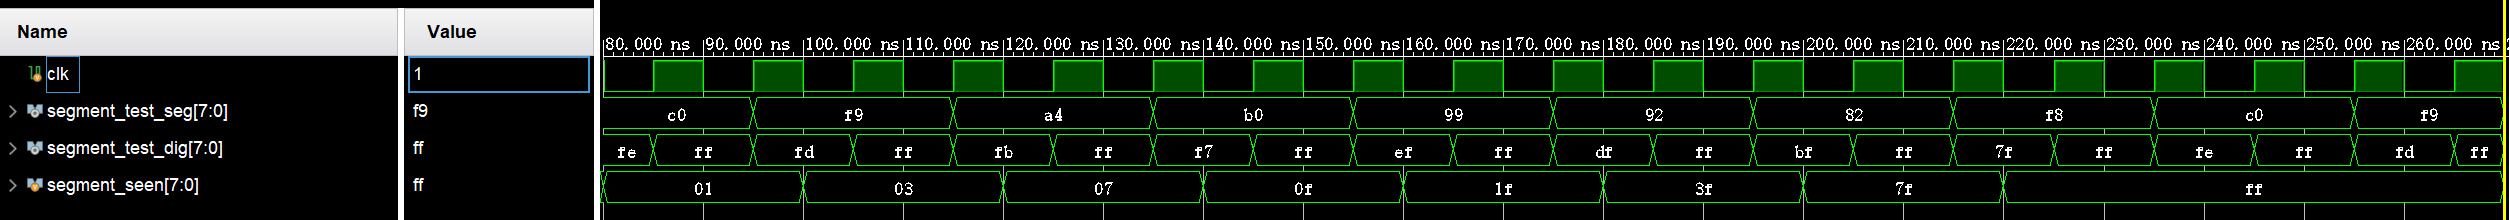
\includegraphics[width=\textwidth]{数码管仿真.png}
    \caption{数码管段码译码与动态扫描仿真结果}
    \label{fig:sim-segment}
\end{figure}

\subsection{日期自动进位验证}

图\ref{fig:sim-january}中，日期由 \signal{1e}、\signal{1f} 递增至
\signal{01}，月份由 \signal{1} 变为 \signal{2}，验证\textbf{1 月末进位}。
图\ref{fig:sim-leap}中，年份保持为 \signal{1c}，日期由 \signal{1c}、
\signal{1d} 进位至 \signal{01}，月份由 \signal{2} 变为 \signal{3}，验证\textbf{闰年 2 月 29 日进位}。

\begin{figure}[H]
    \centering
    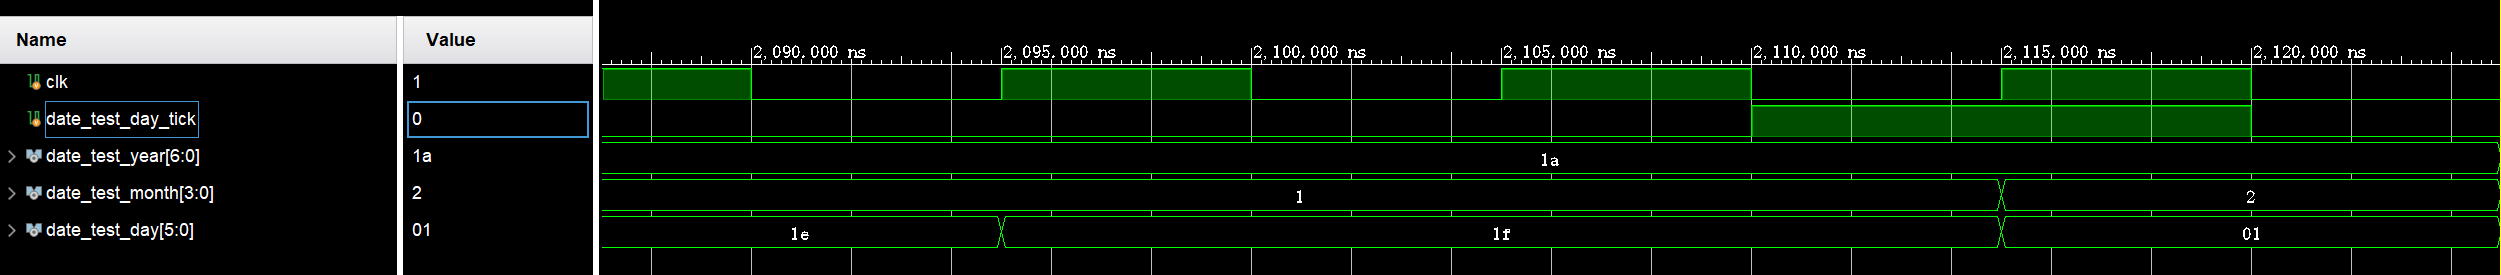
\includegraphics[width=\textwidth]{1月进位.png}
    \caption{1 月末日期自动进位仿真结果}
    \label{fig:sim-january}
\end{figure}

\begin{figure}[H]
    \centering
    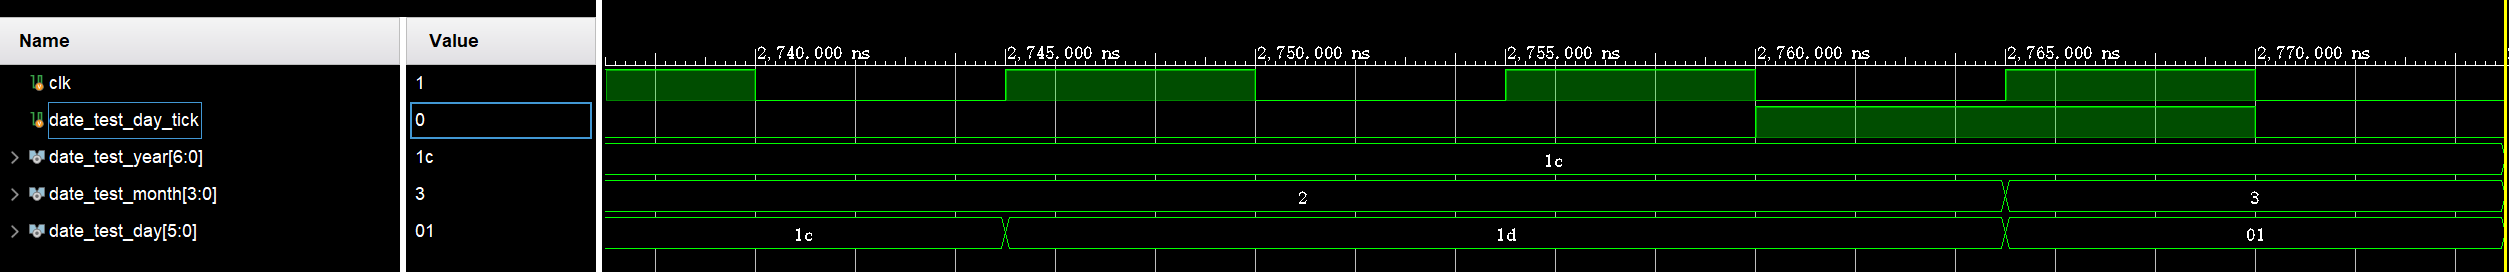
\includegraphics[width=\textwidth]{闰年进位.png}
    \caption{闰年 2 月 29 日自动进位仿真结果}
    \label{fig:sim-leap}
\end{figure}

\subsection{倒计时结束提示验证}

图\ref{fig:sim-countdown}中，倒计时由 \signal{00:01} 变为 \signal{00:00} 后，
\signal{countdown_test_finish} 保持有效\textbf{5 个逻辑秒}；在此期间
\signal{countdown_test_led} 连续翻转，完成\textbf{结束提醒}。

\begin{figure}[H]
    \centering
    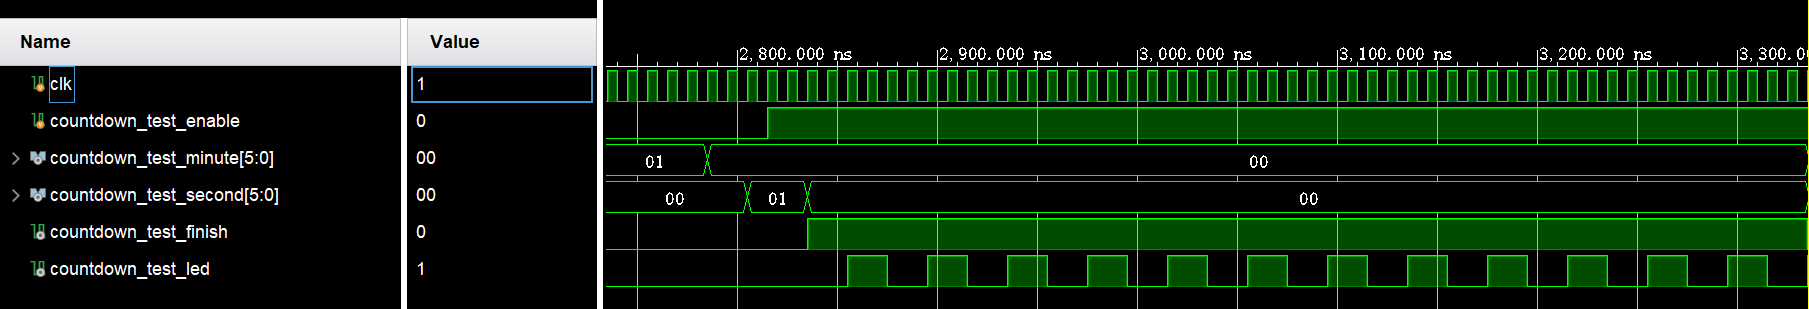
\includegraphics[width=\textwidth]{倒计时测试.png}
    \caption{倒计时结束提示与 LED 闪烁仿真结果}
    \label{fig:sim-countdown}
\end{figure}

\subsection{闹钟二次提醒验证}

图\ref{fig:sim-alarm-repeat}中，\signal{alarm_test_trigger} 首次有效后自动撤销，
等待\textbf{10 个逻辑秒}后再次有效，验证闹钟的\textbf{二次提醒流程}。

\begin{figure}[H]
    \centering
    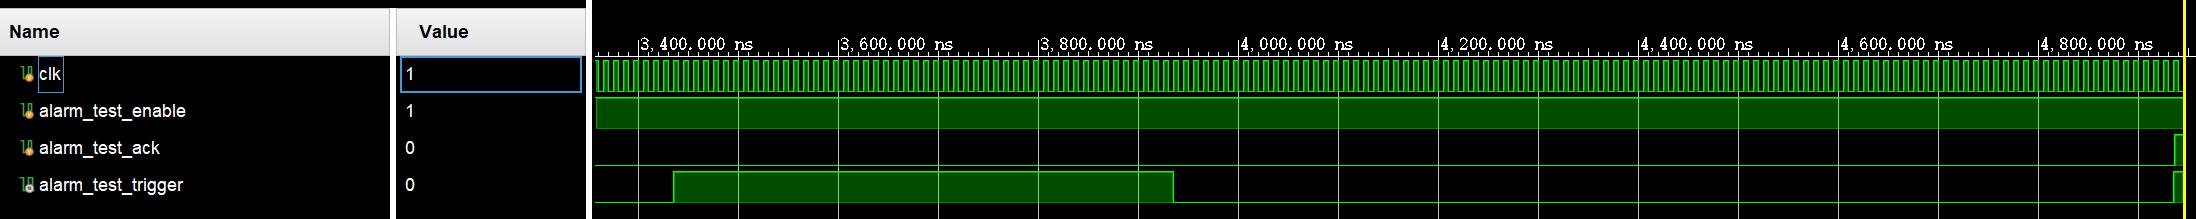
\includegraphics[width=\textwidth]{闹钟_1.png}
    \caption{闹钟首次提醒、等待与二次提醒仿真结果}
    \label{fig:sim-alarm-repeat}
\end{figure}

\subsection{闹钟确认关闭验证}

图\ref{fig:sim-alarm-ack}中，\signal{alarm_test_ack} 产生确认脉冲后，
\signal{alarm_test_trigger} 随即清零，验证用户确认后可\textbf{关闭当前提醒}。

\begin{figure}[H]
    \centering
    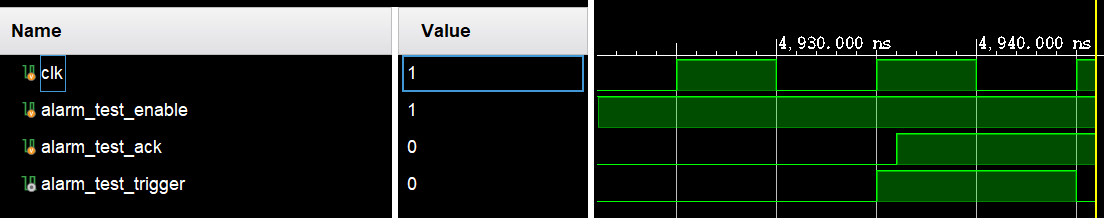
\includegraphics[width=0.75\textwidth]{闹钟_2.png}
    \caption{闹钟确认关闭仿真结果}
    \label{fig:sim-alarm-ack}
\end{figure}

\section{板级验证}

系统在 HX7A75C FPGA 开发板上验证，板载 50 MHz 时钟接入 \signal{clk}。
\signal{clock.xdc} 完成 4 个低电平有效按键、4 个拨码开关、八位数码管与
LED1 的管脚约束。使用 Vivado 2023.2 生成并下载 \signal{clock_top.bit}。以数码管正放为准，
验证时将 \signal{SW6} 拨下连接数码管，\signal{SW1}--\signal{SW4} 初始拨上。

\subsection{页面显示与切换验证}

图\ref{fig:board-pages}给出时间、日期、闹钟和倒计时页面的实际显示结果。
按 \signal{KEY1} 可在四个页面间\textbf{循环切换}，显示内容与设计格式一致。

\begin{figure}[H]
    \centering
    \begin{minipage}[t]{0.23\textwidth}
        \centering
        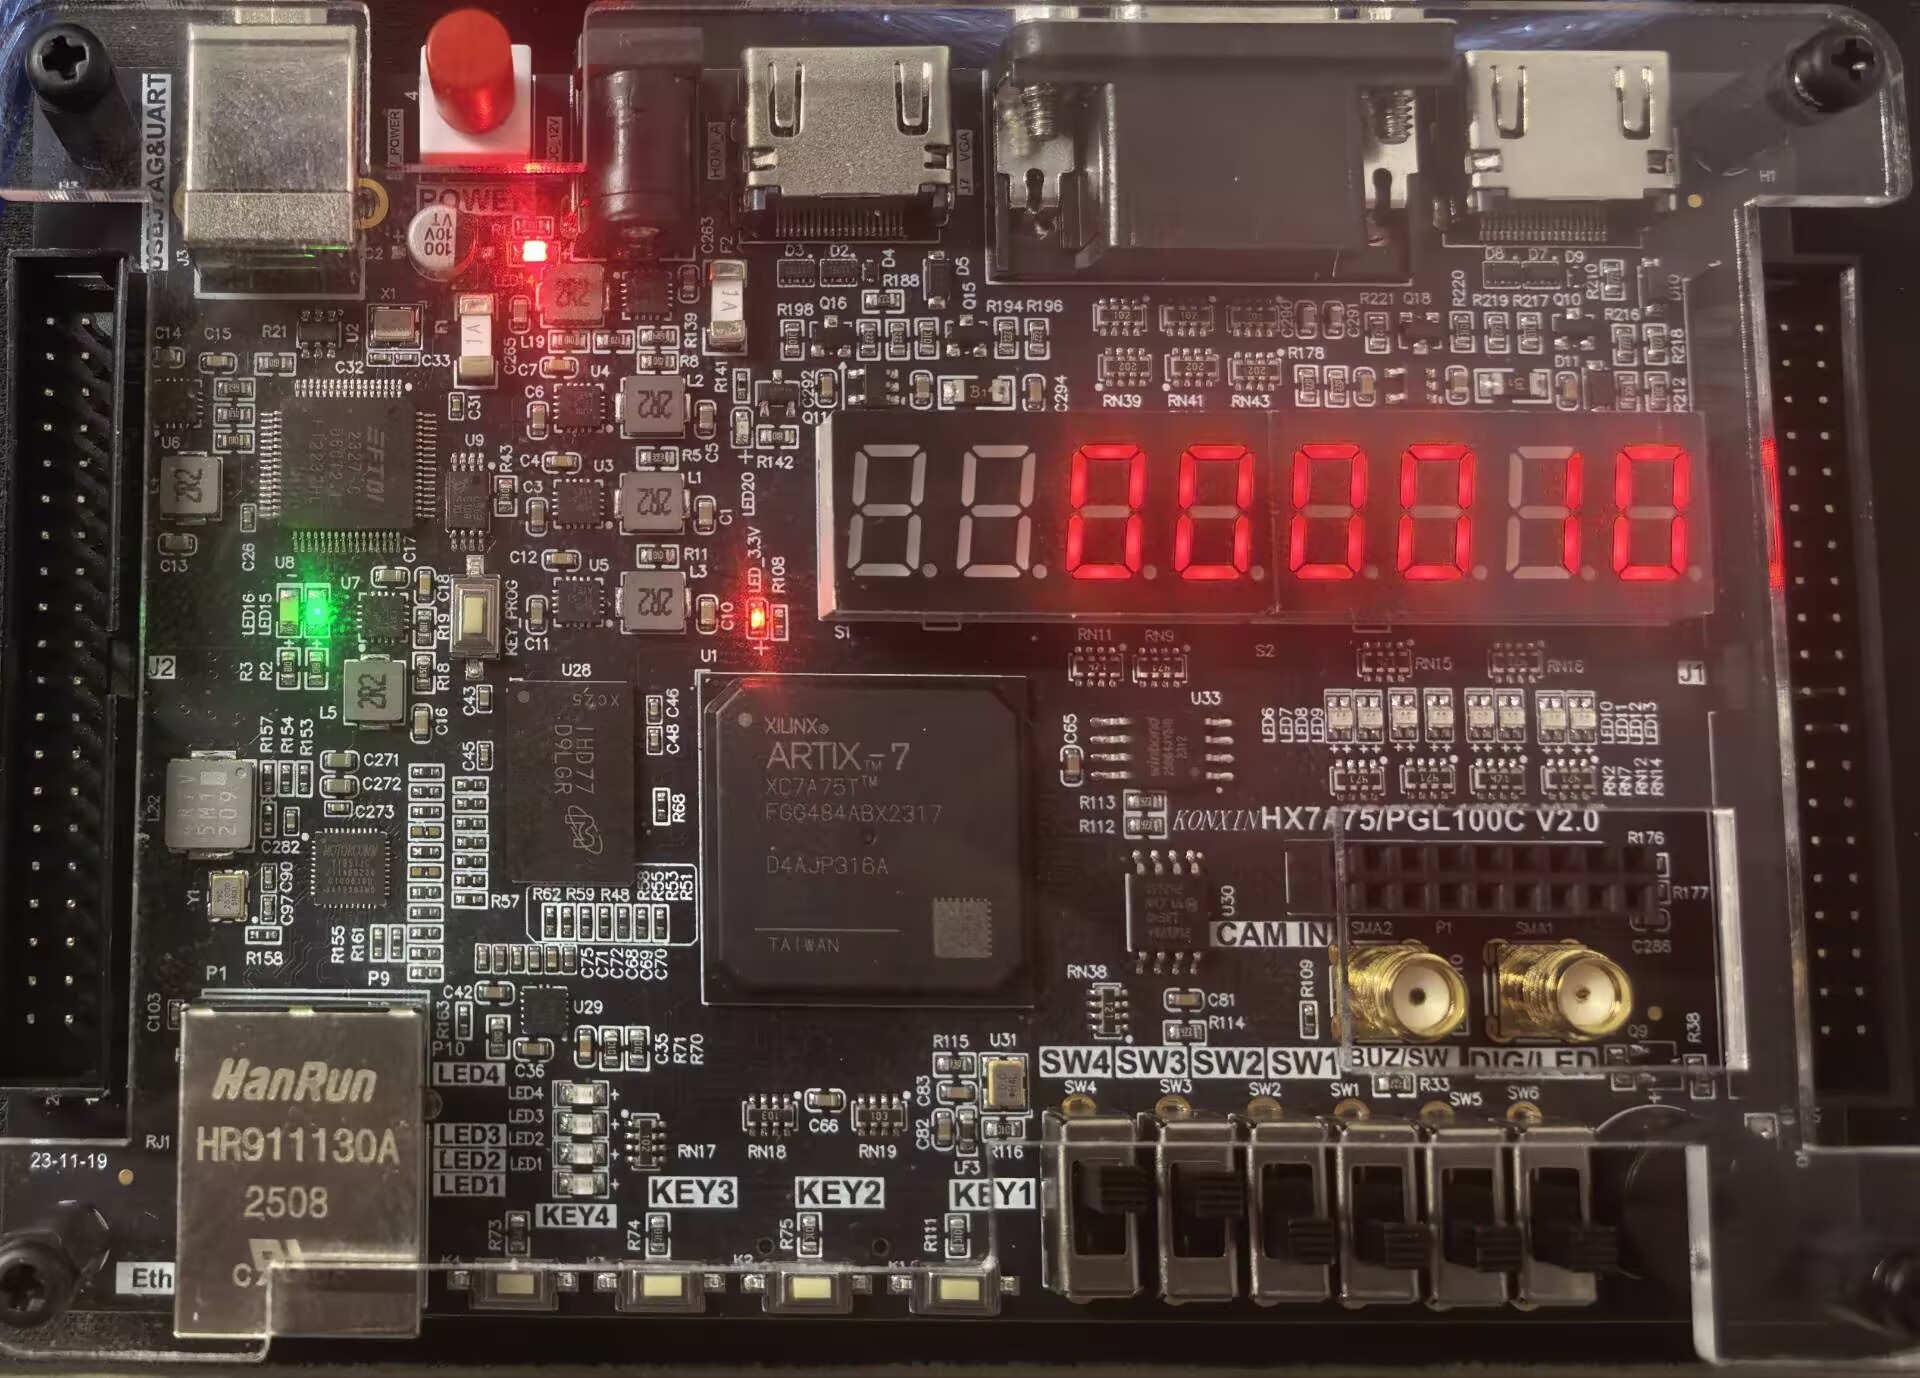
\includegraphics[width=\linewidth]{时间000010.jpg}\\[-1mm]
        \scriptsize (a) 时间页
    \end{minipage}\hfill
    \begin{minipage}[t]{0.23\textwidth}
        \centering
        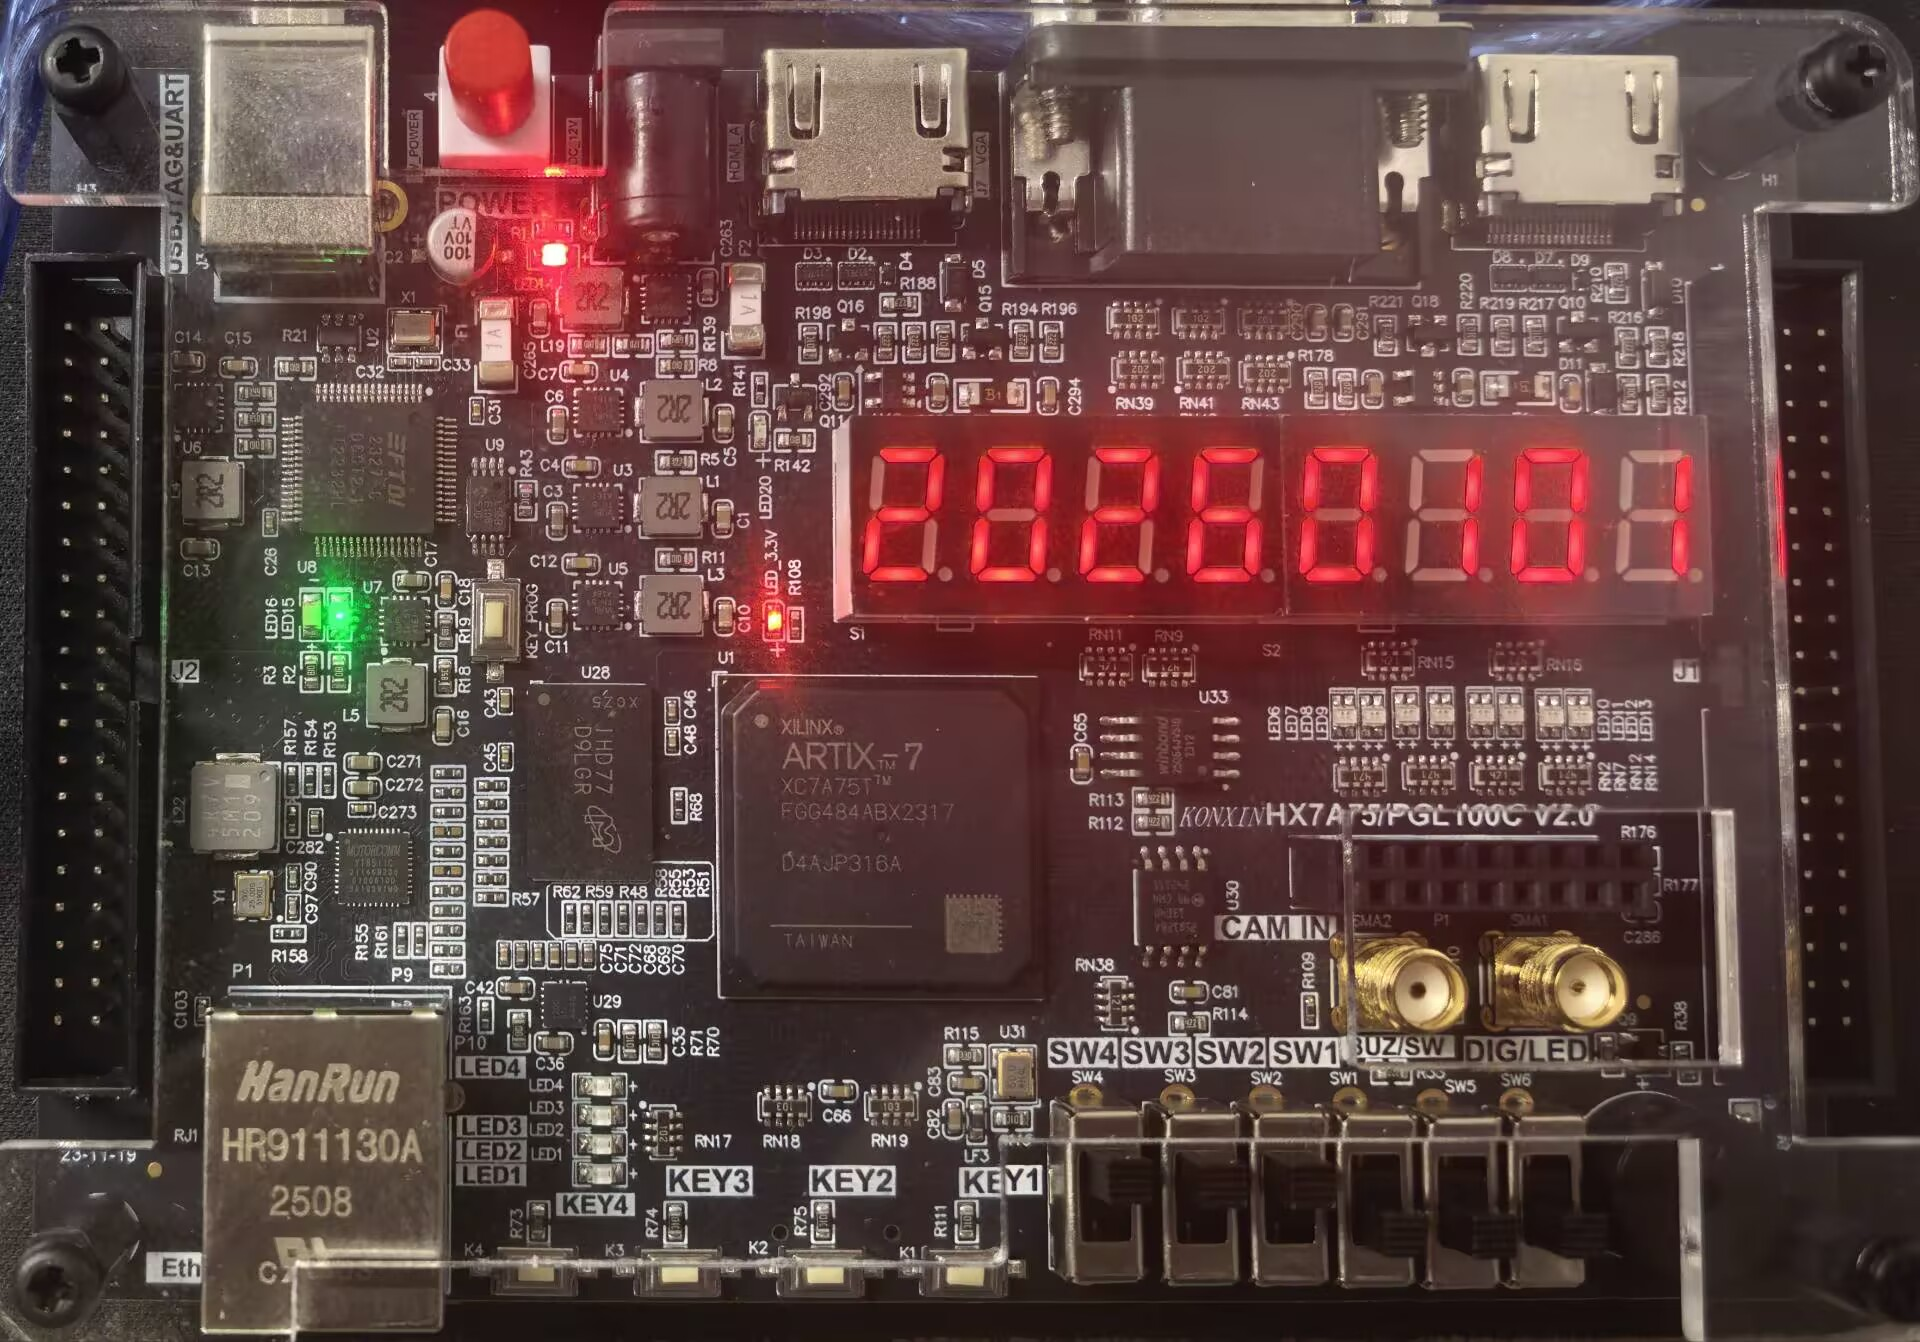
\includegraphics[width=\linewidth]{日期20260101.jpg}\\[-1mm]
        \scriptsize (b) 日期页
    \end{minipage}\hfill
    \begin{minipage}[t]{0.23\textwidth}
        \centering
        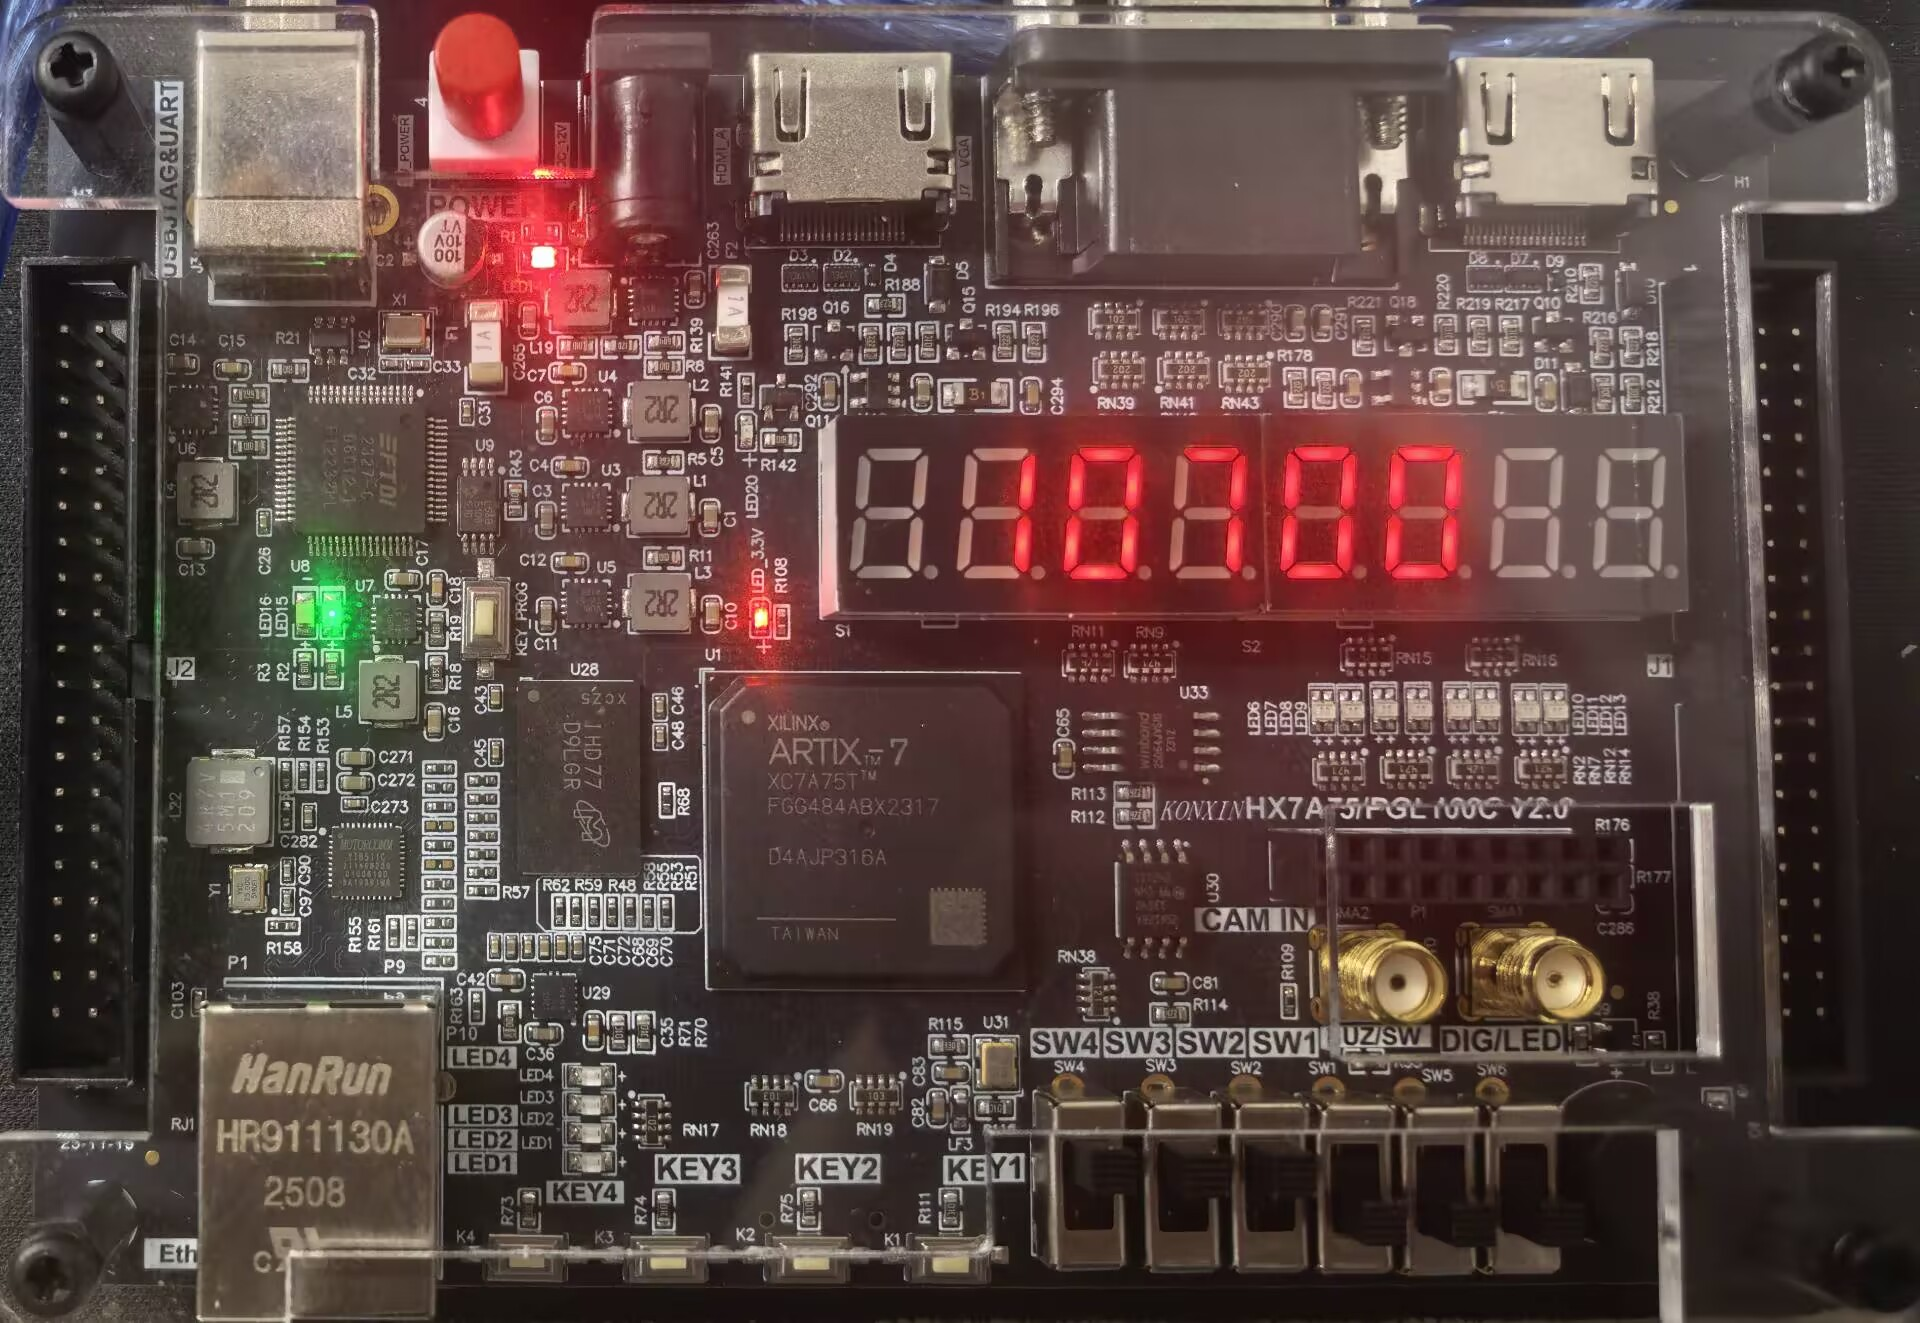
\includegraphics[width=\linewidth]{闹钟10700.jpg}\\[-1mm]
        \scriptsize (c) 闹钟页
    \end{minipage}\hfill
    \begin{minipage}[t]{0.23\textwidth}
        \centering
        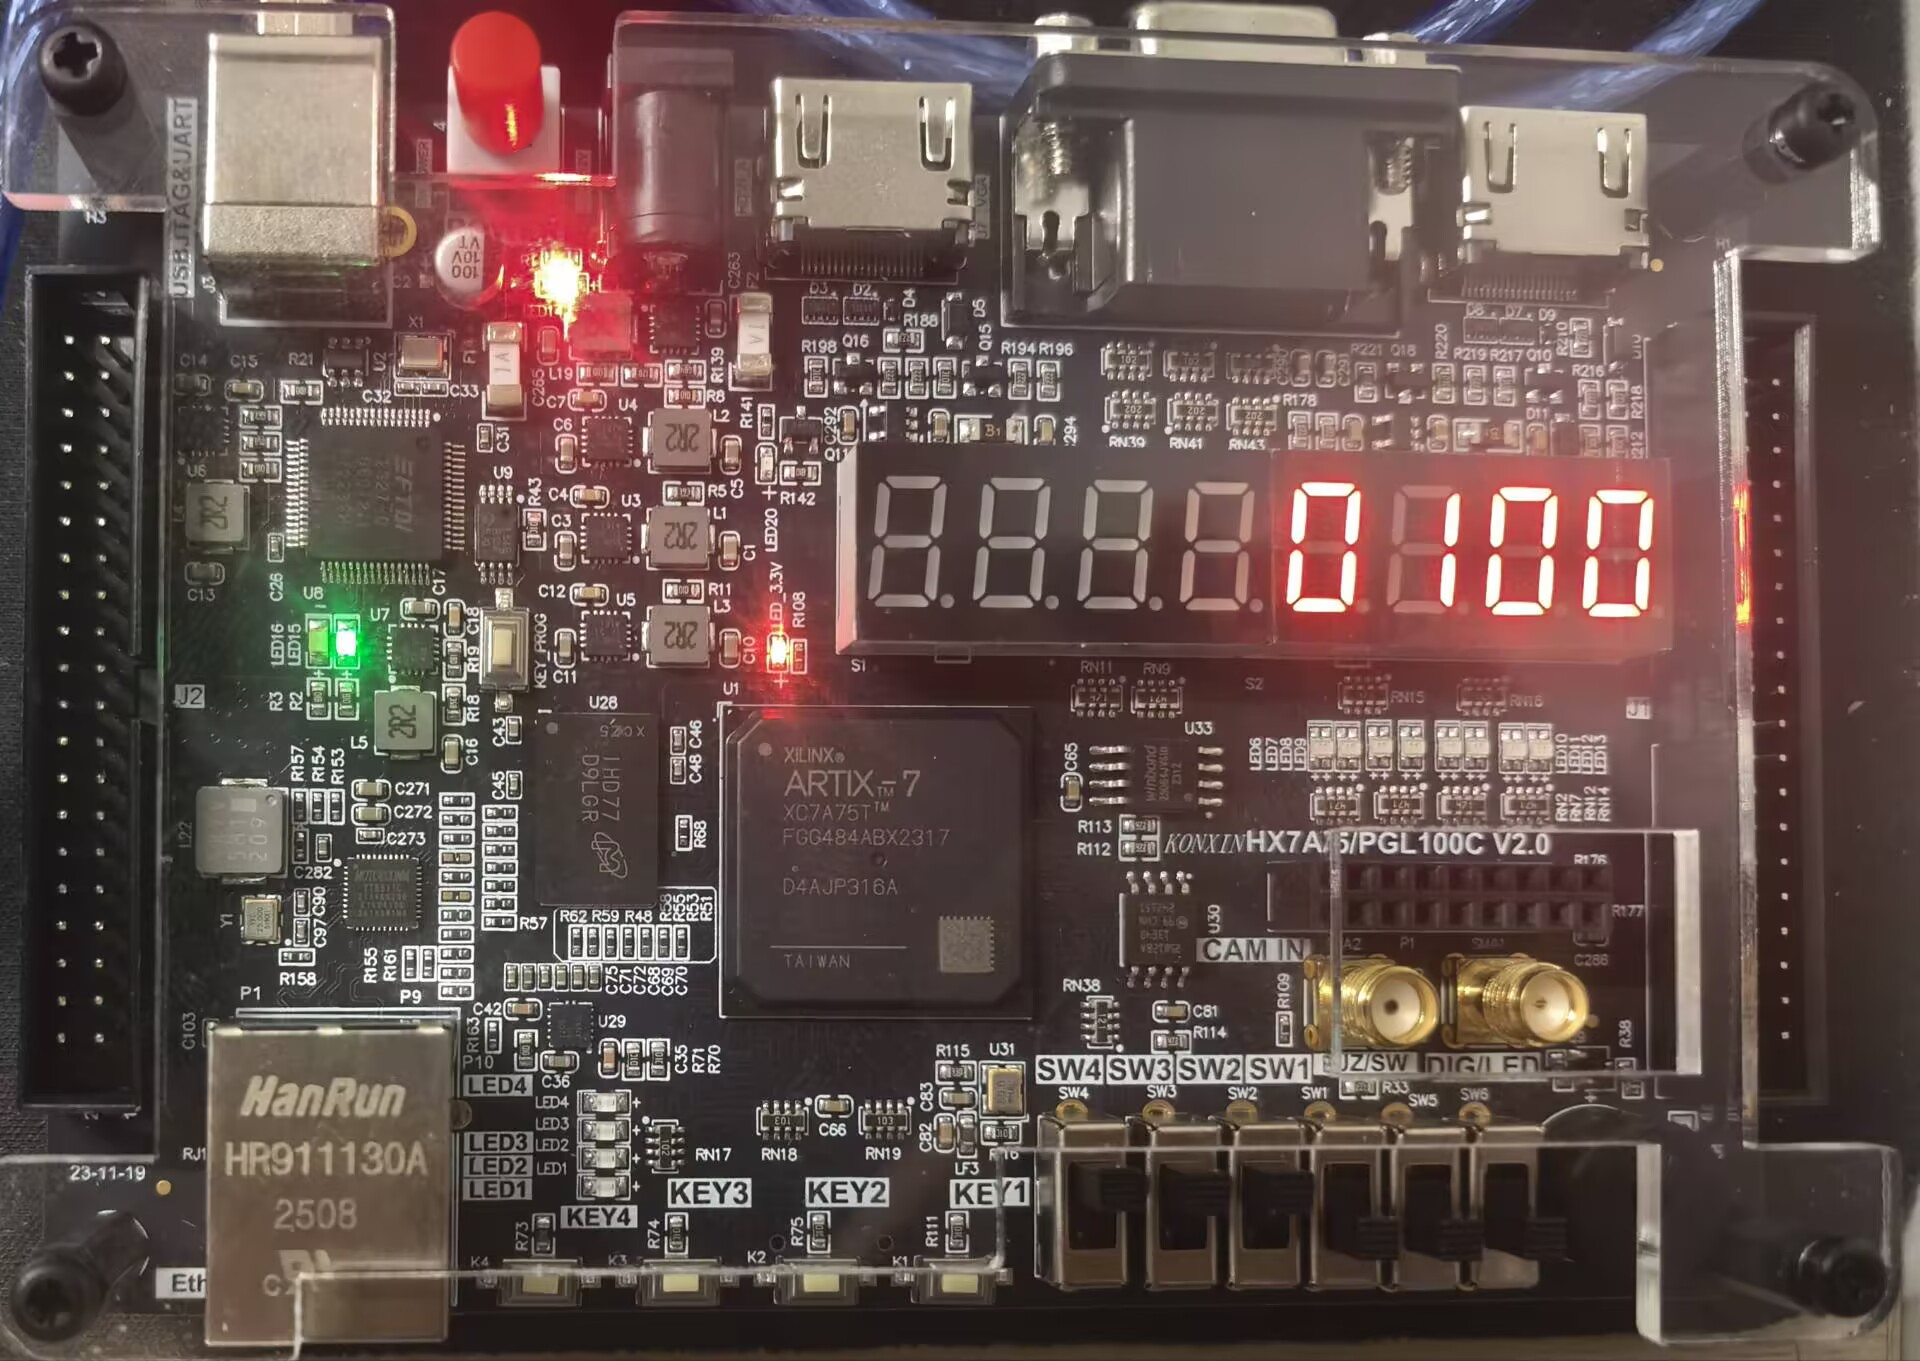
\includegraphics[width=\linewidth]{倒计时0010.jpg}\\[-1mm]
        \scriptsize (d) 倒计时页
    \end{minipage}
    \caption{四个页面的板级显示结果}
\label{fig:board-pages}
\end{figure}

\subsection{倒计时结束提示验证}

倒计时页面进入修改模式后可设置初值；退出修改模式并启动后，数码管递减至
\signal{00:00}，\textbf{LED1 亮起并闪烁}，结果如图\ref{fig:board-countdown}所示。

\begin{figure}[H]
    \centering
    \begin{minipage}[t]{0.42\textwidth}
        \centering
        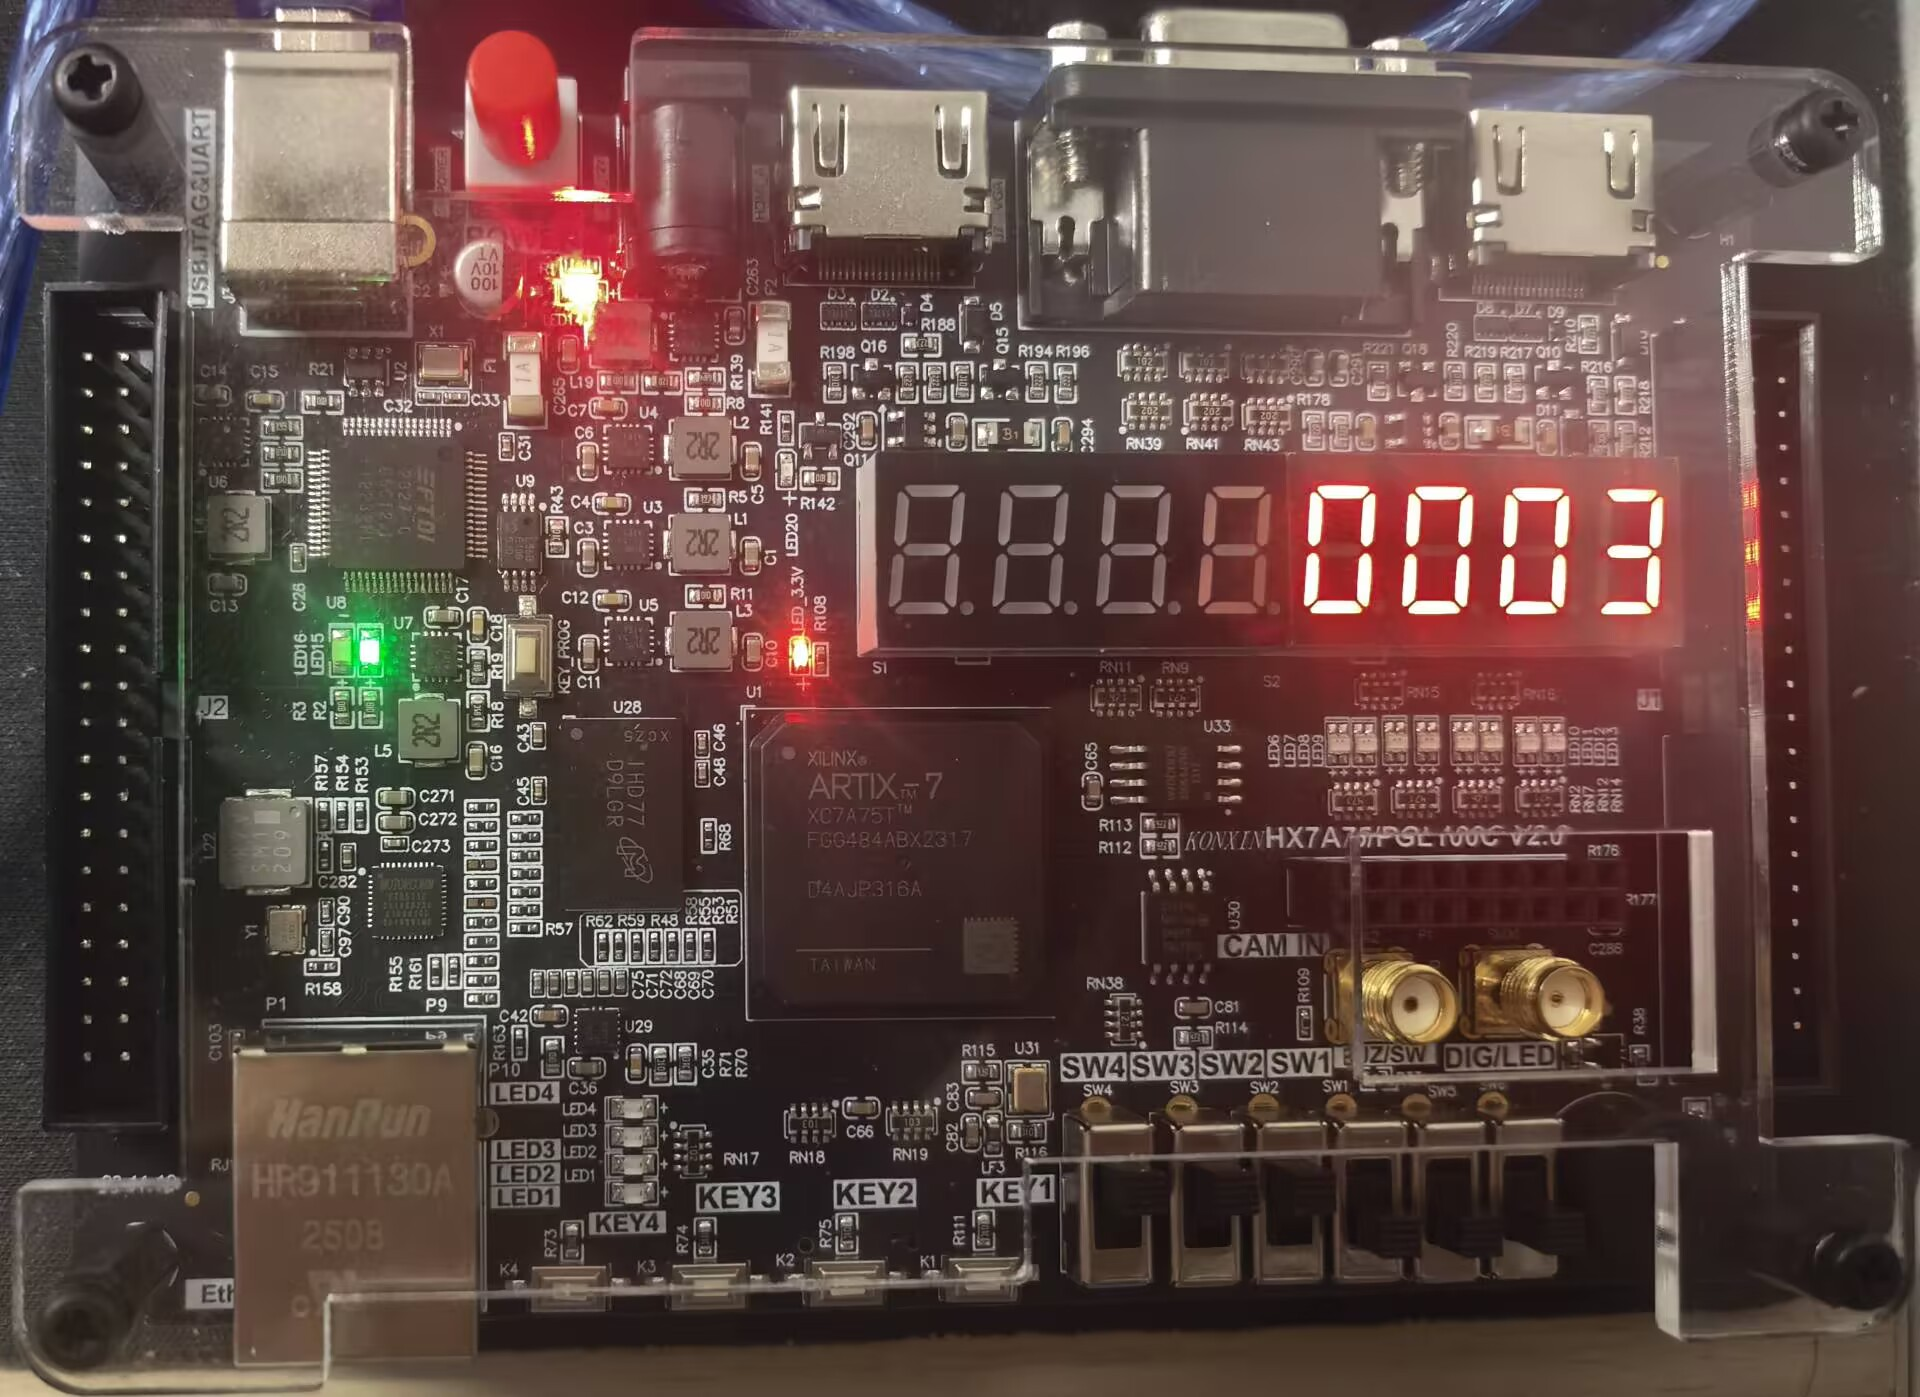
\includegraphics[width=\linewidth]{倒计时调整0003.jpg}\\[-1mm]
        \small (a) 修改为 \signal{00:03}
    \end{minipage}\hfill
    \begin{minipage}[t]{0.42\textwidth}
        \centering
        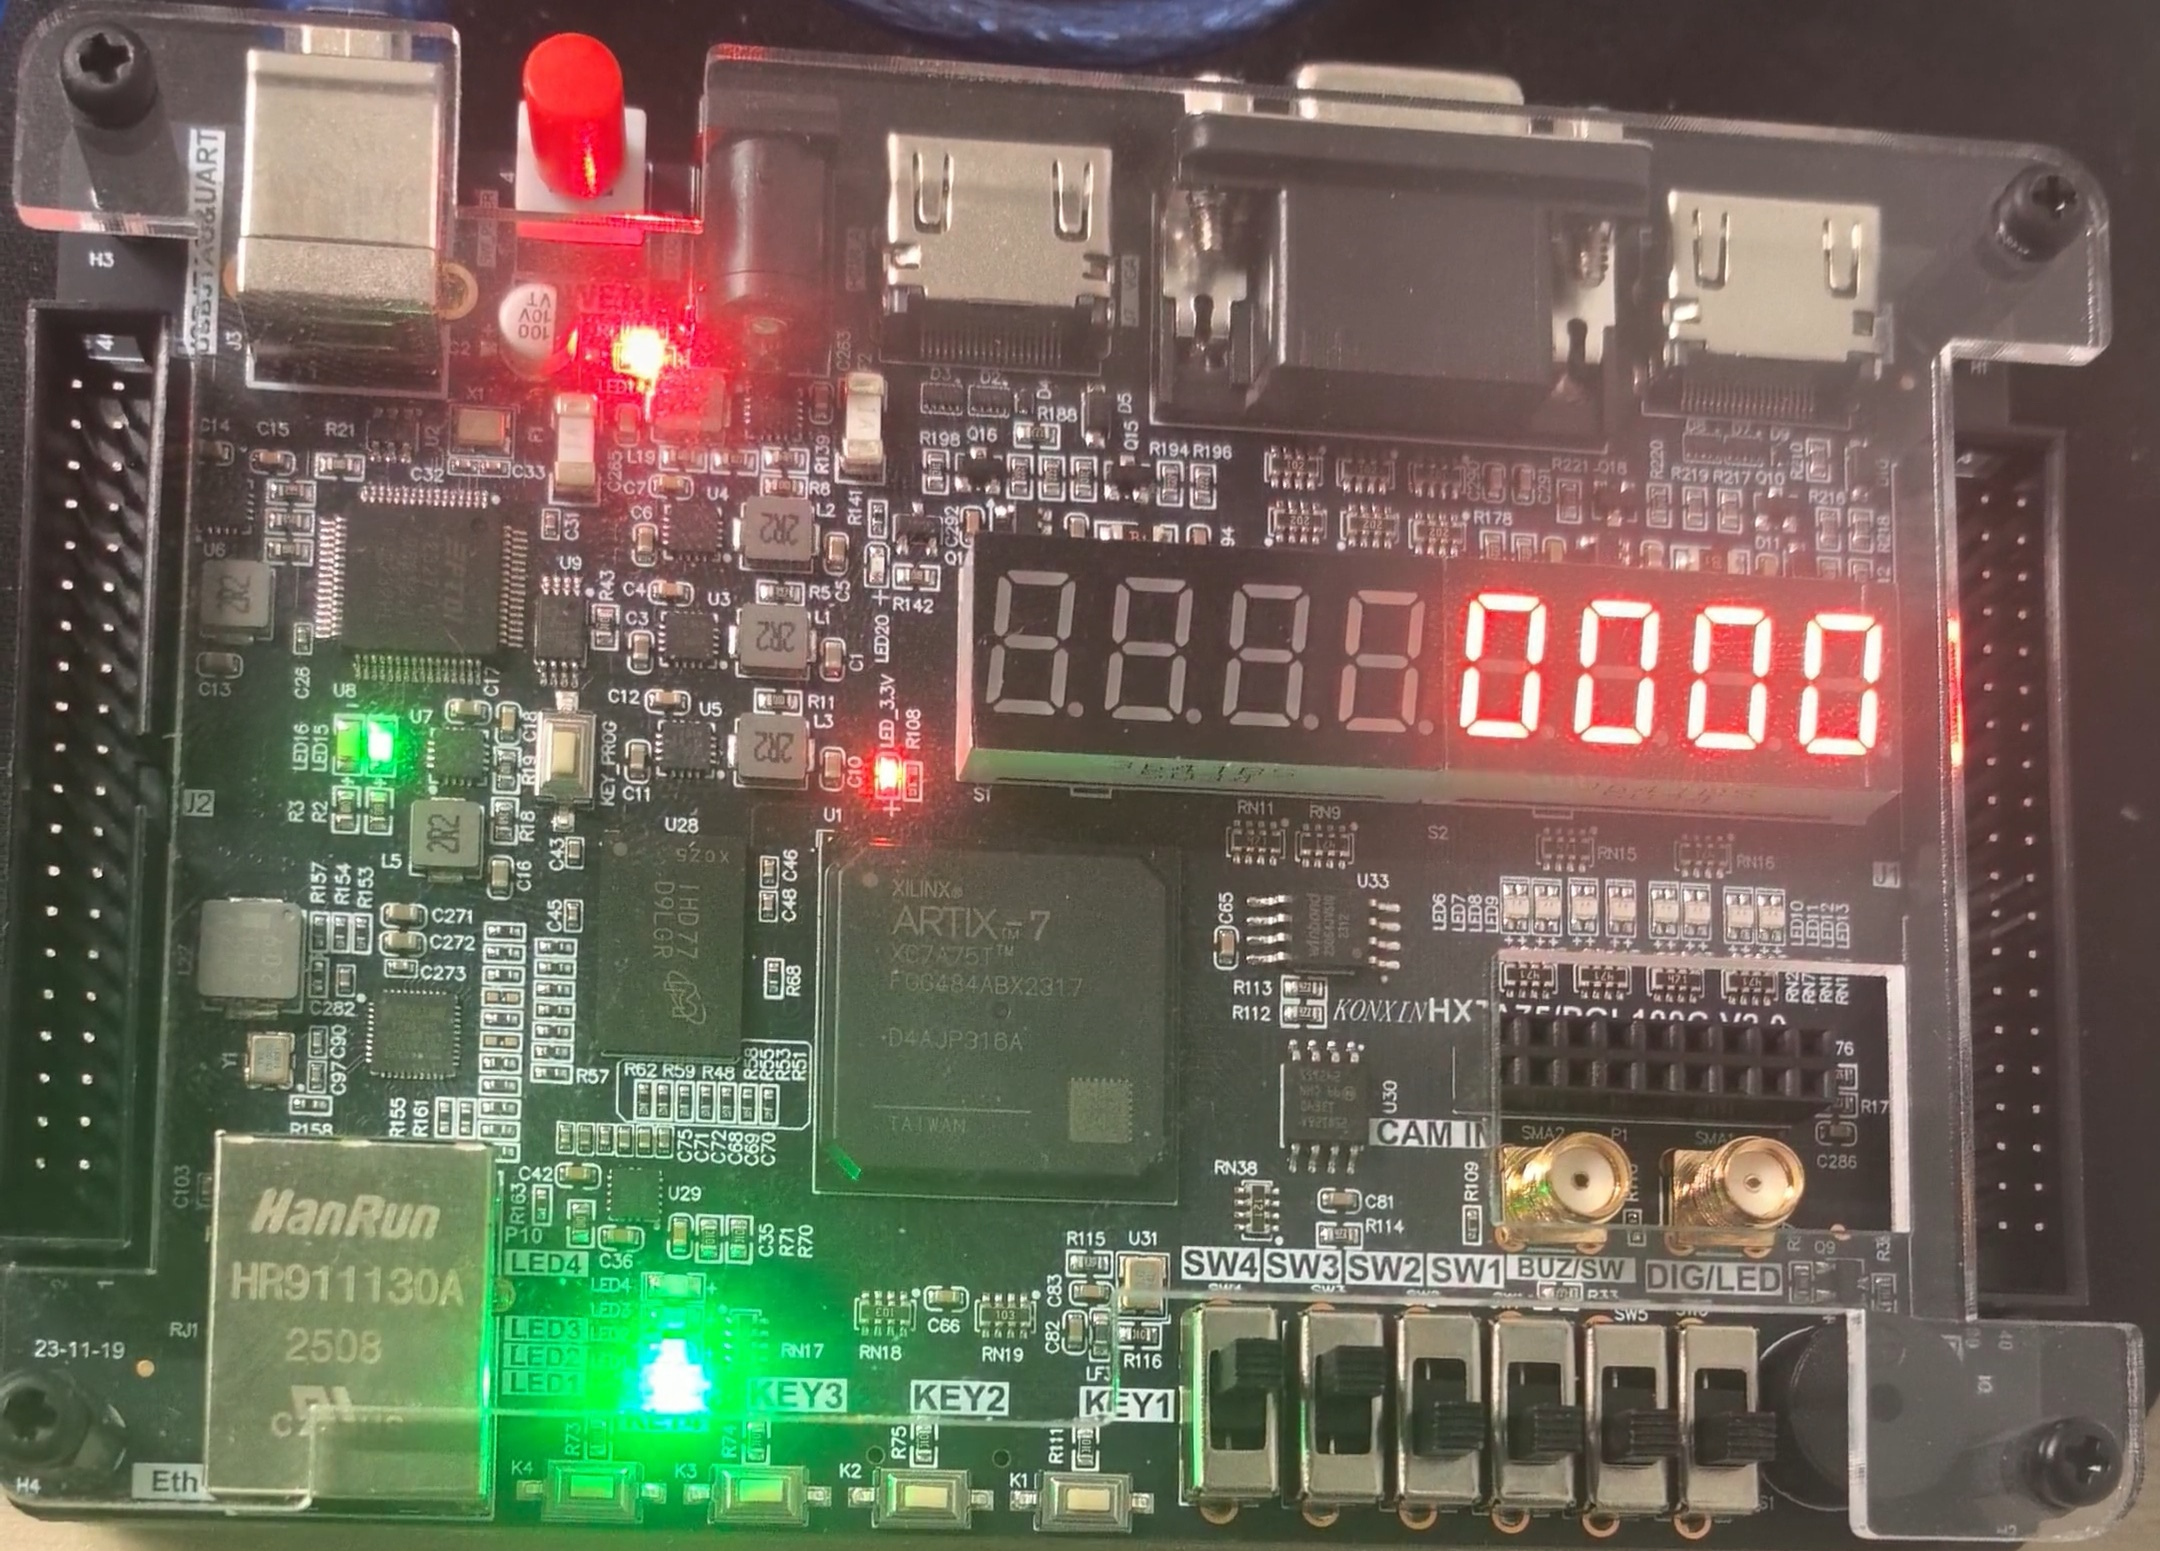
\includegraphics[width=\linewidth]{倒计时结束0000LED亮.jpeg}\\[-1mm]
        \small (b) 归零并触发 LED1 提醒
    \end{minipage}
    \caption{倒计时设置与结束提醒的板级验证}
\label{fig:board-countdown}
\end{figure}

\subsection{闹钟提醒与确认关闭验证}

将闹钟设置为 \signal{00:01} 并开启闹钟后，\textbf{首次提醒、二次提醒}及
\signal{KEY4} 确认关闭的板级结果如图\ref{fig:board-alarm}所示。

\begin{figure}[H]
    \centering
    \begin{minipage}[t]{0.30\textwidth}
        \centering
        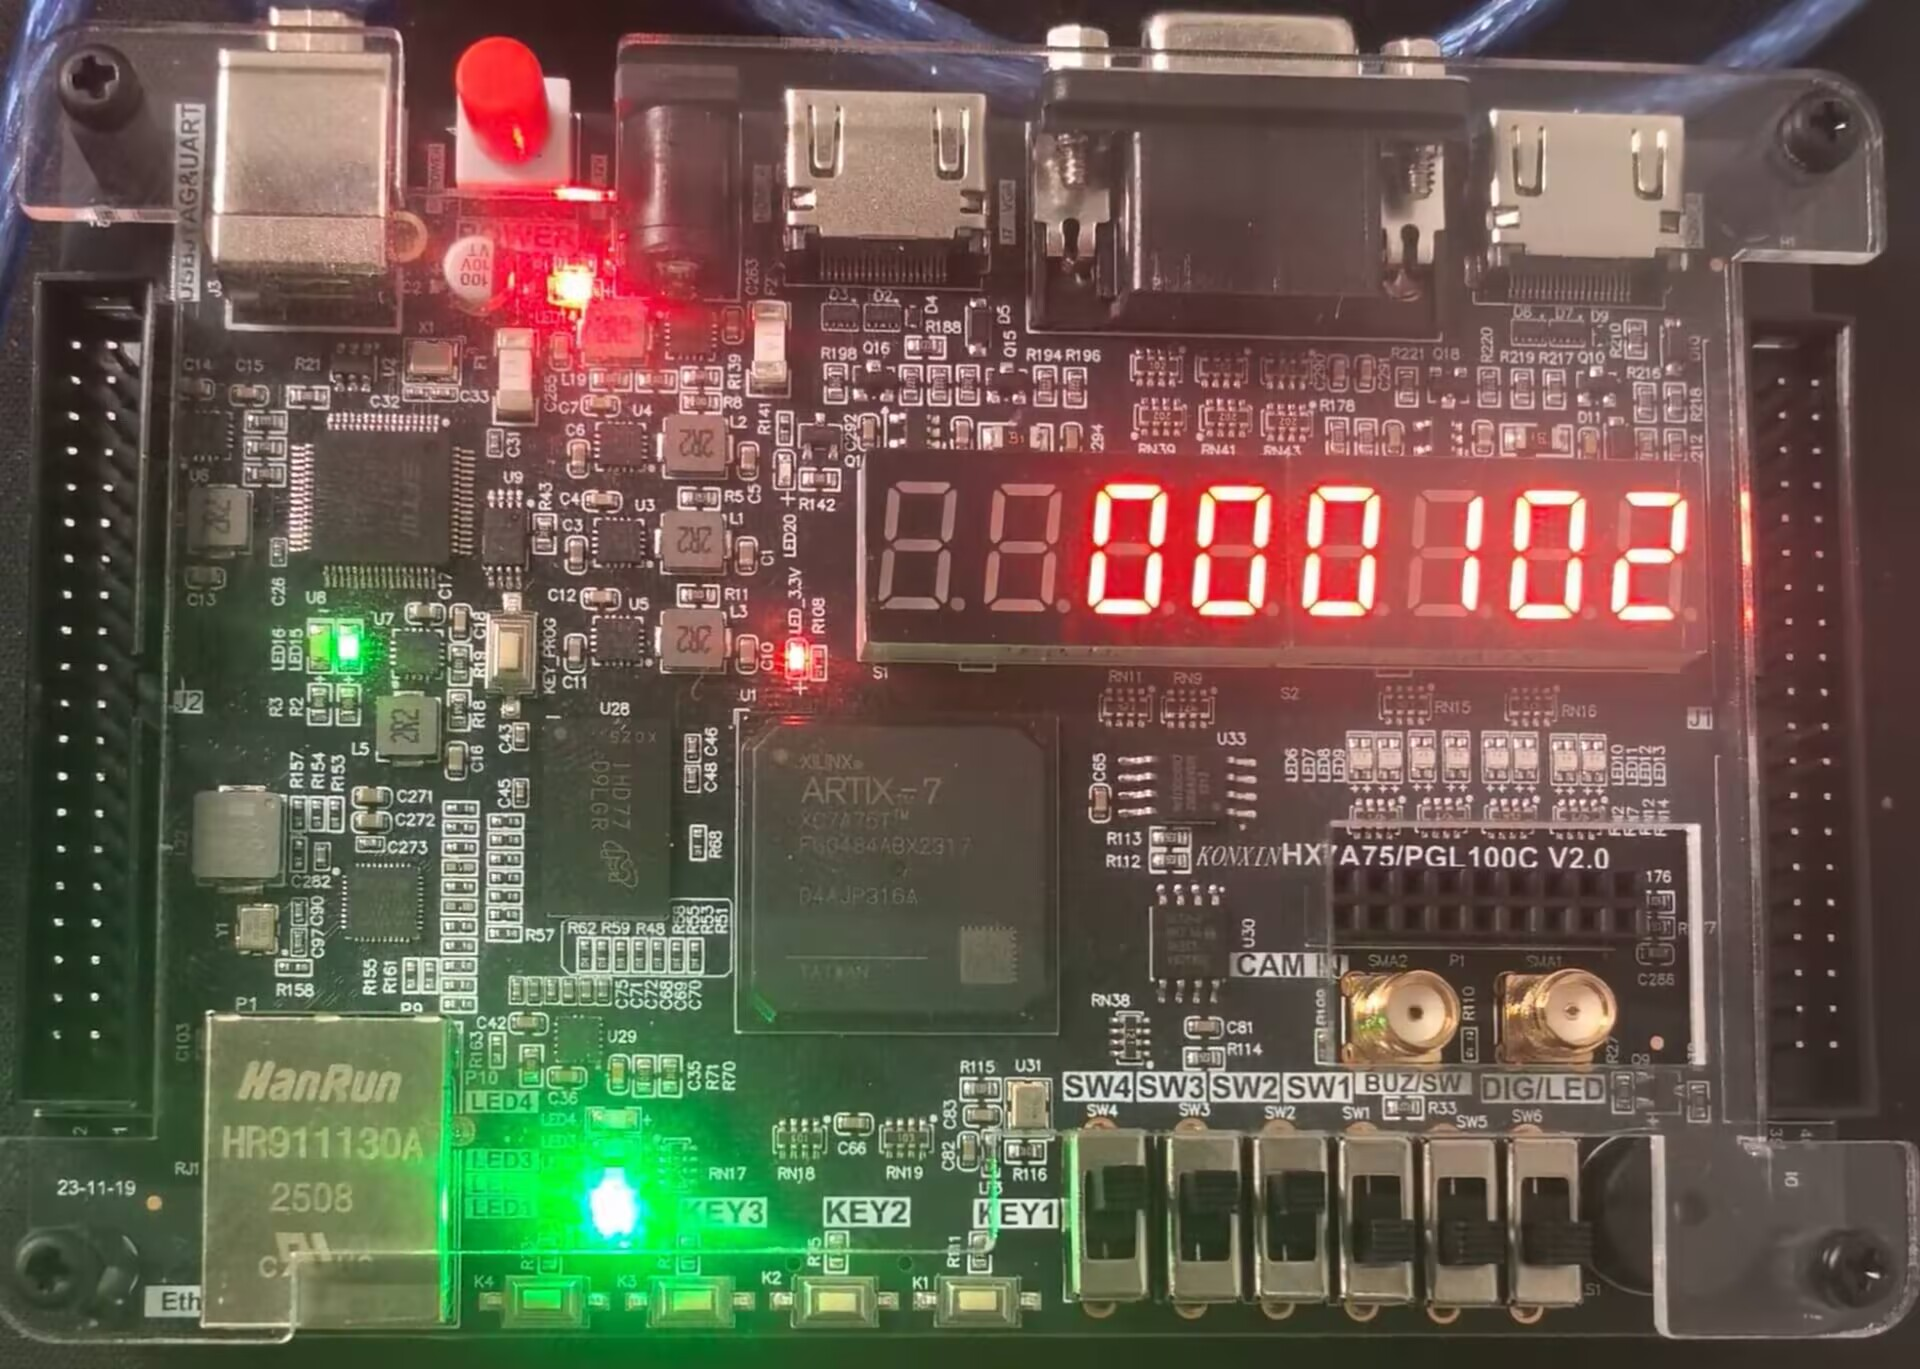
\includegraphics[width=\linewidth]{000100闹钟首次响铃亮拍照时为000102.jpg}\\[-1mm]
        \scriptsize (a) 首次提醒，LED1 亮
    \end{minipage}\hfill
    \begin{minipage}[t]{0.30\textwidth}
        \centering
        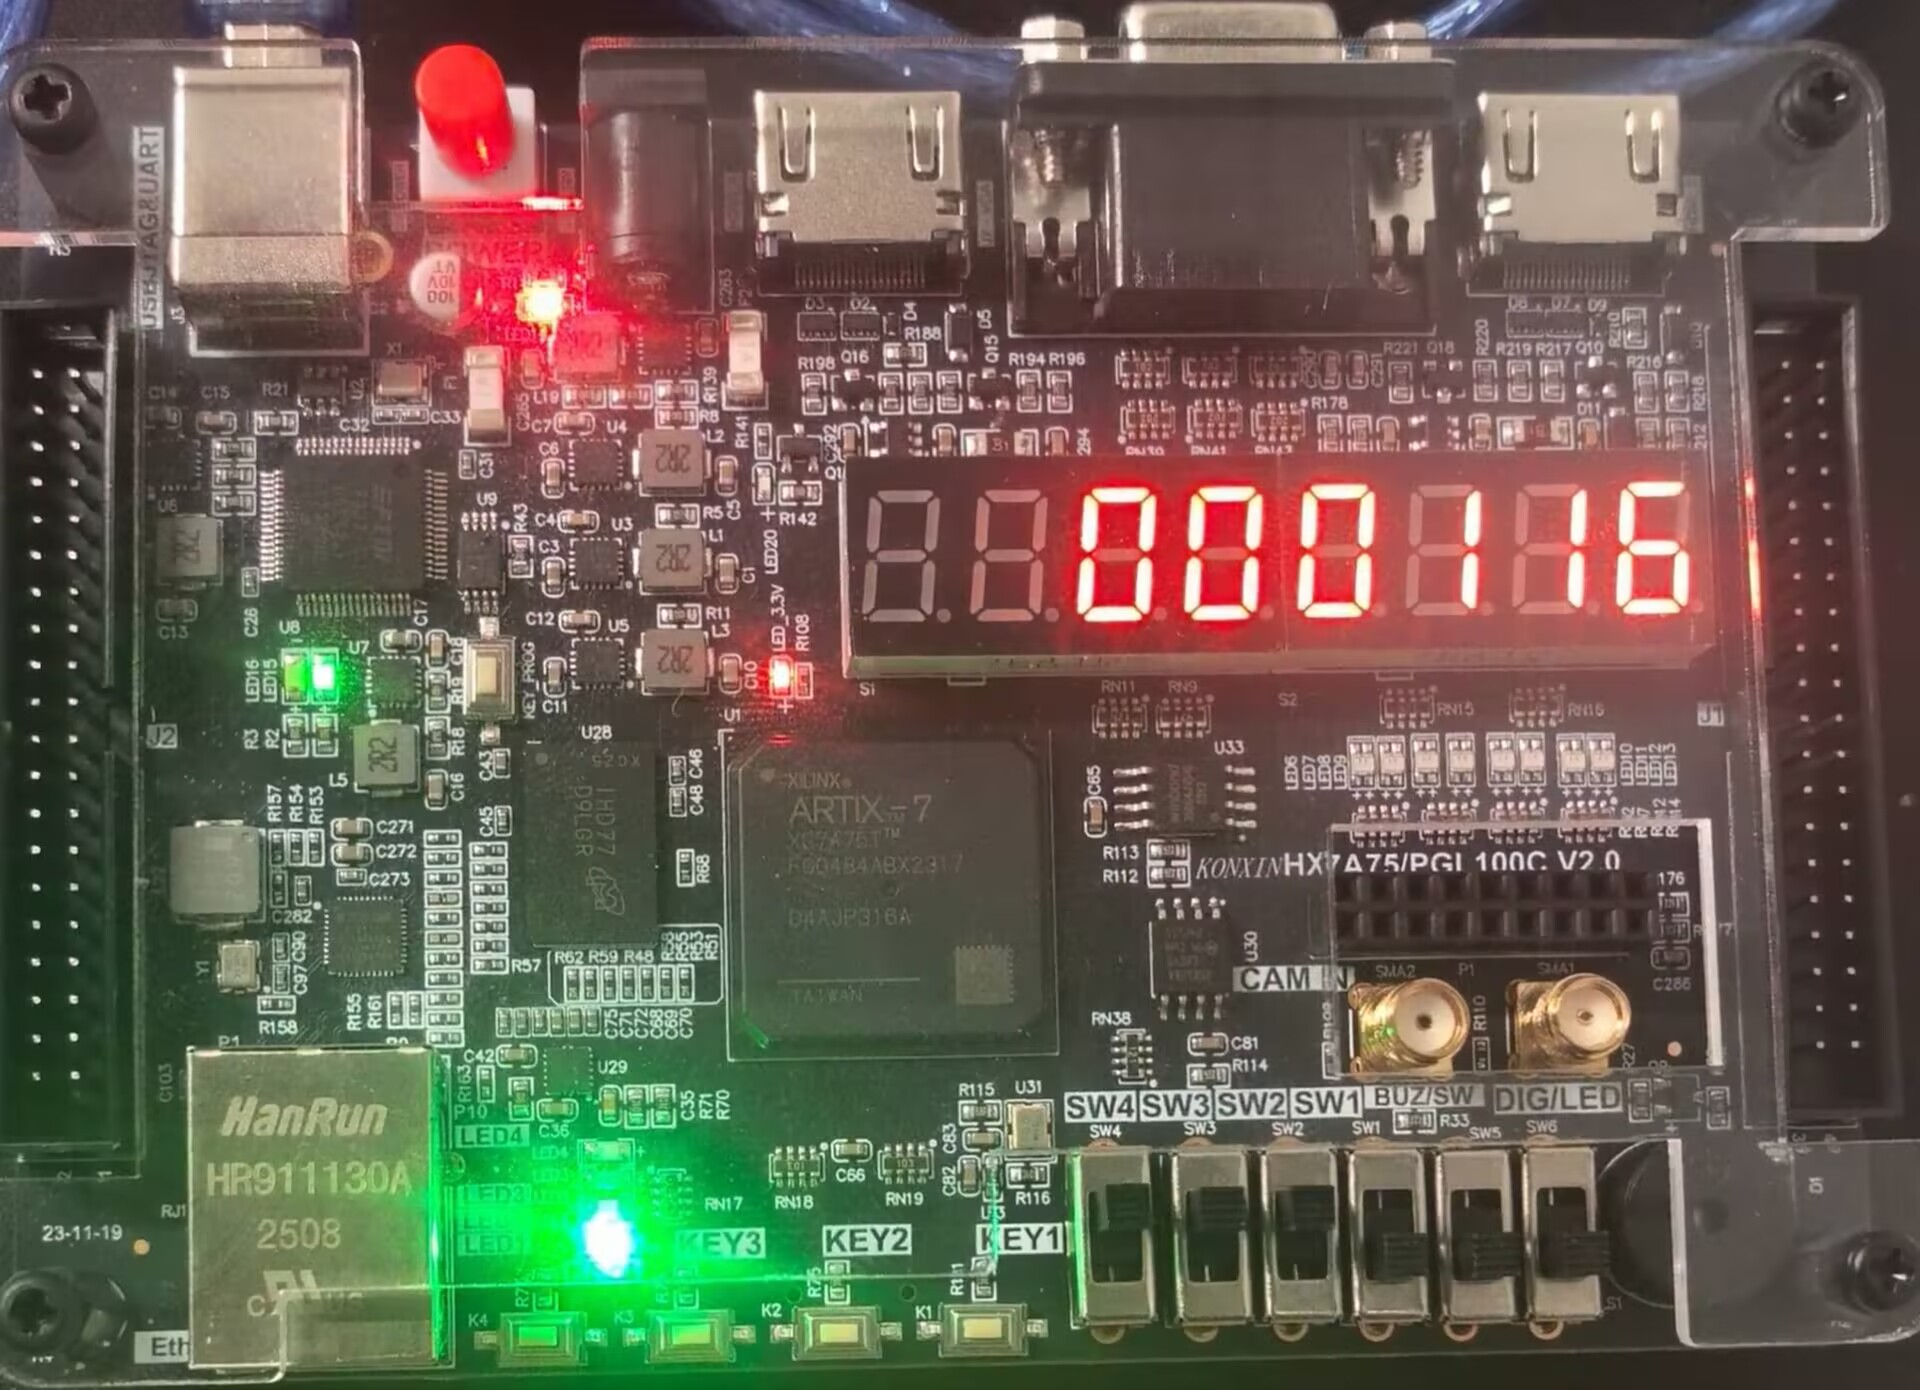
\includegraphics[width=\linewidth]{闹钟延迟10秒再次响铃并亮LED此时000116.jpg}\\[-1mm]
        \scriptsize (b) 二次提醒，LED1 亮
    \end{minipage}\hfill
    \begin{minipage}[t]{0.30\textwidth}
        \centering
        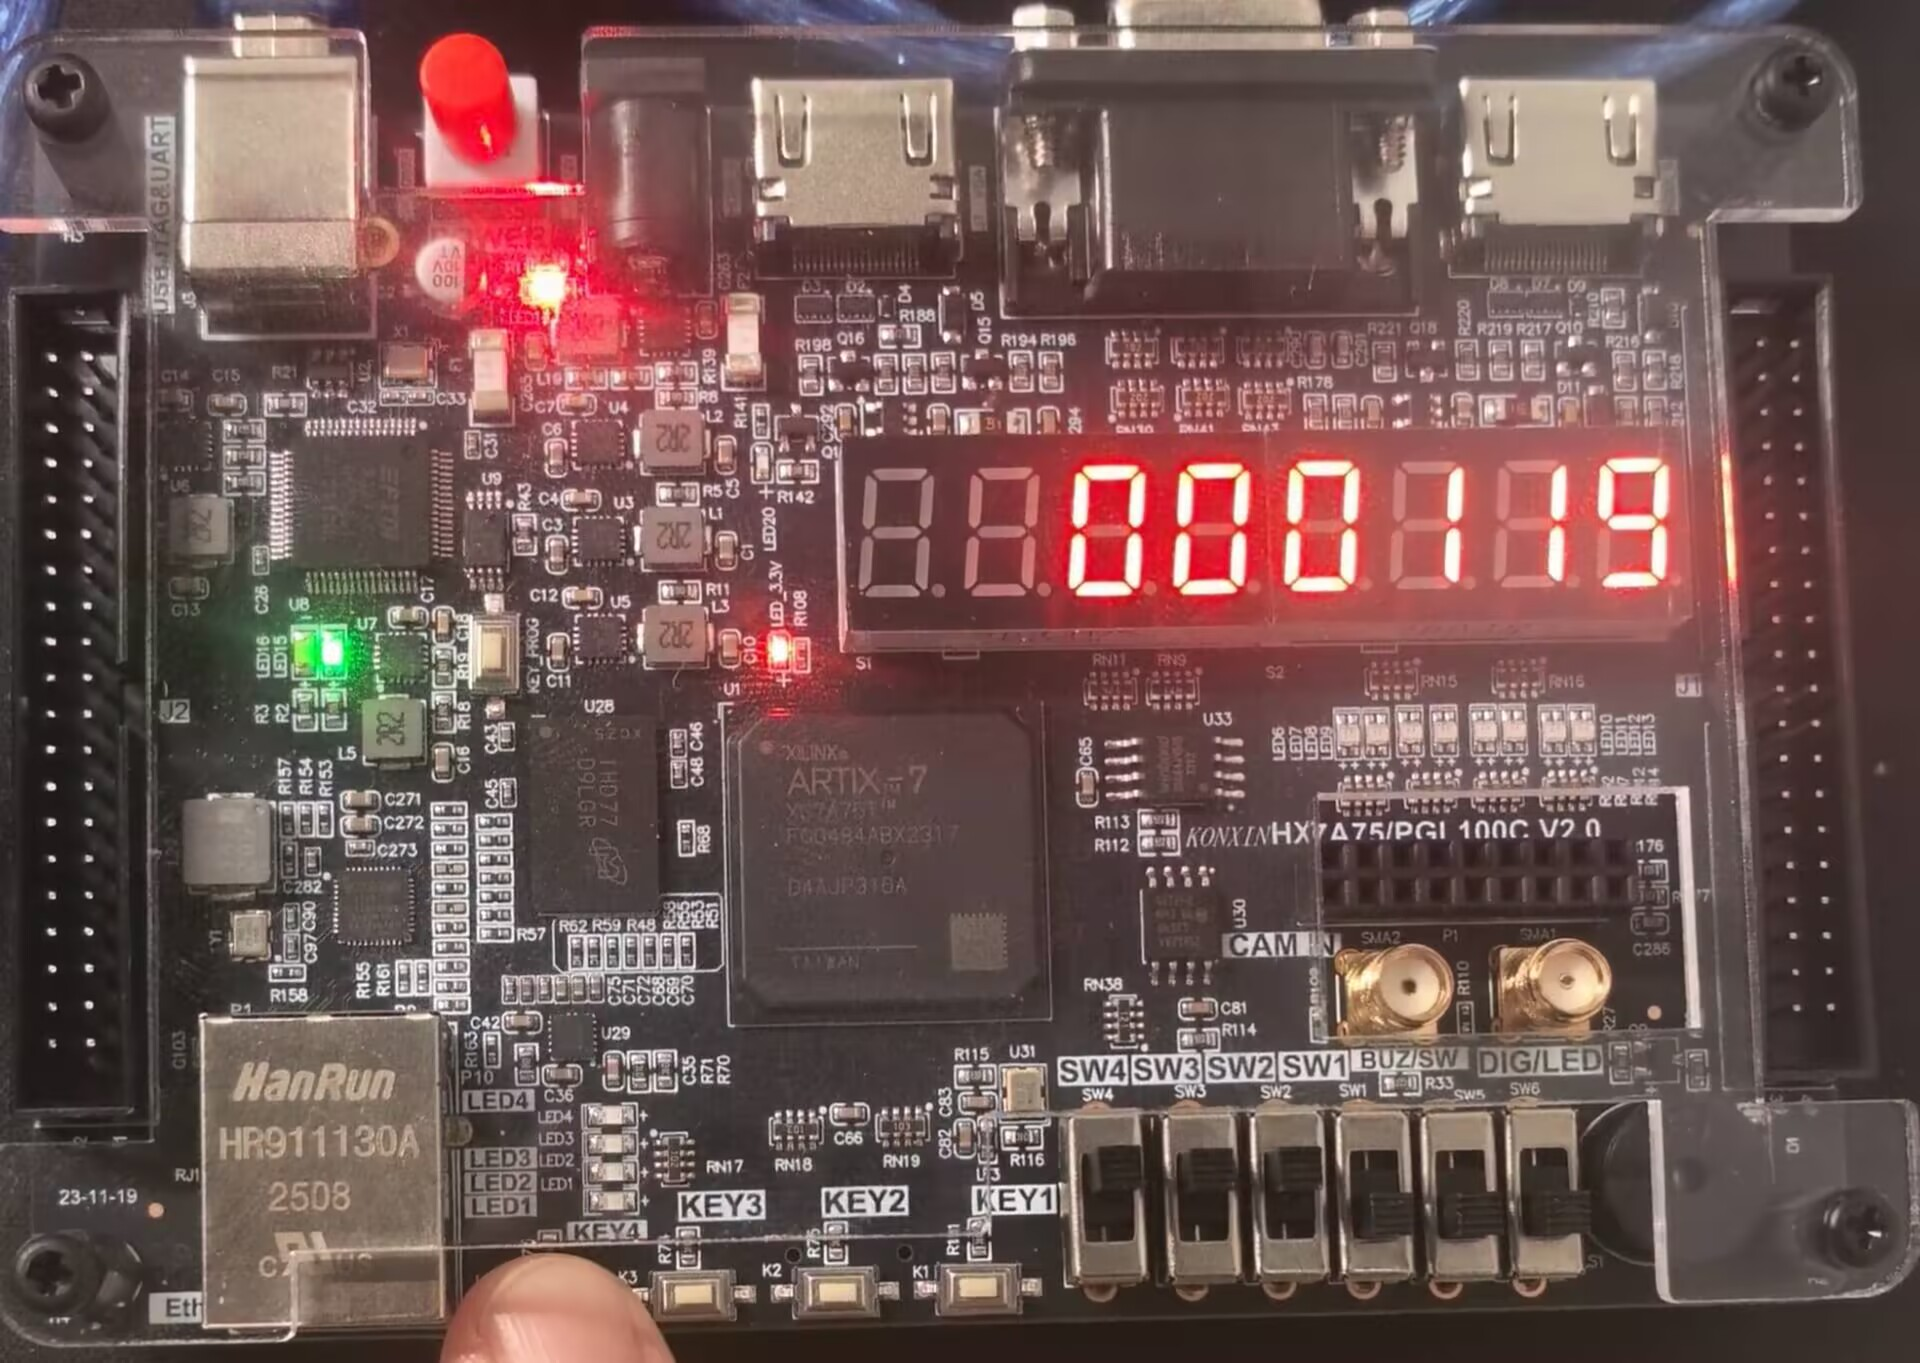
\includegraphics[width=\linewidth]{闹钟摁下确认键LED灭此时000119.jpg}\\[-1mm]
        \scriptsize (c) \signal{KEY4} 确认后 LED1 灭
    \end{minipage}
    \caption{闹钟提醒与确认关闭的板级验证}
\label{fig:board-alarm}
\end{figure}

\subsection{全局复位验证}

\textbf{全局复位}由 \signal{SW4} 拨下后按 \signal{KEY4} 触发。图\ref{fig:board-reset}
在同一行展示复位前、显示全灭、恢复扫描和复位完成四个状态。

\begin{figure}[H]
    \centering
    \begin{minipage}[t]{0.23\textwidth}
        \centering
        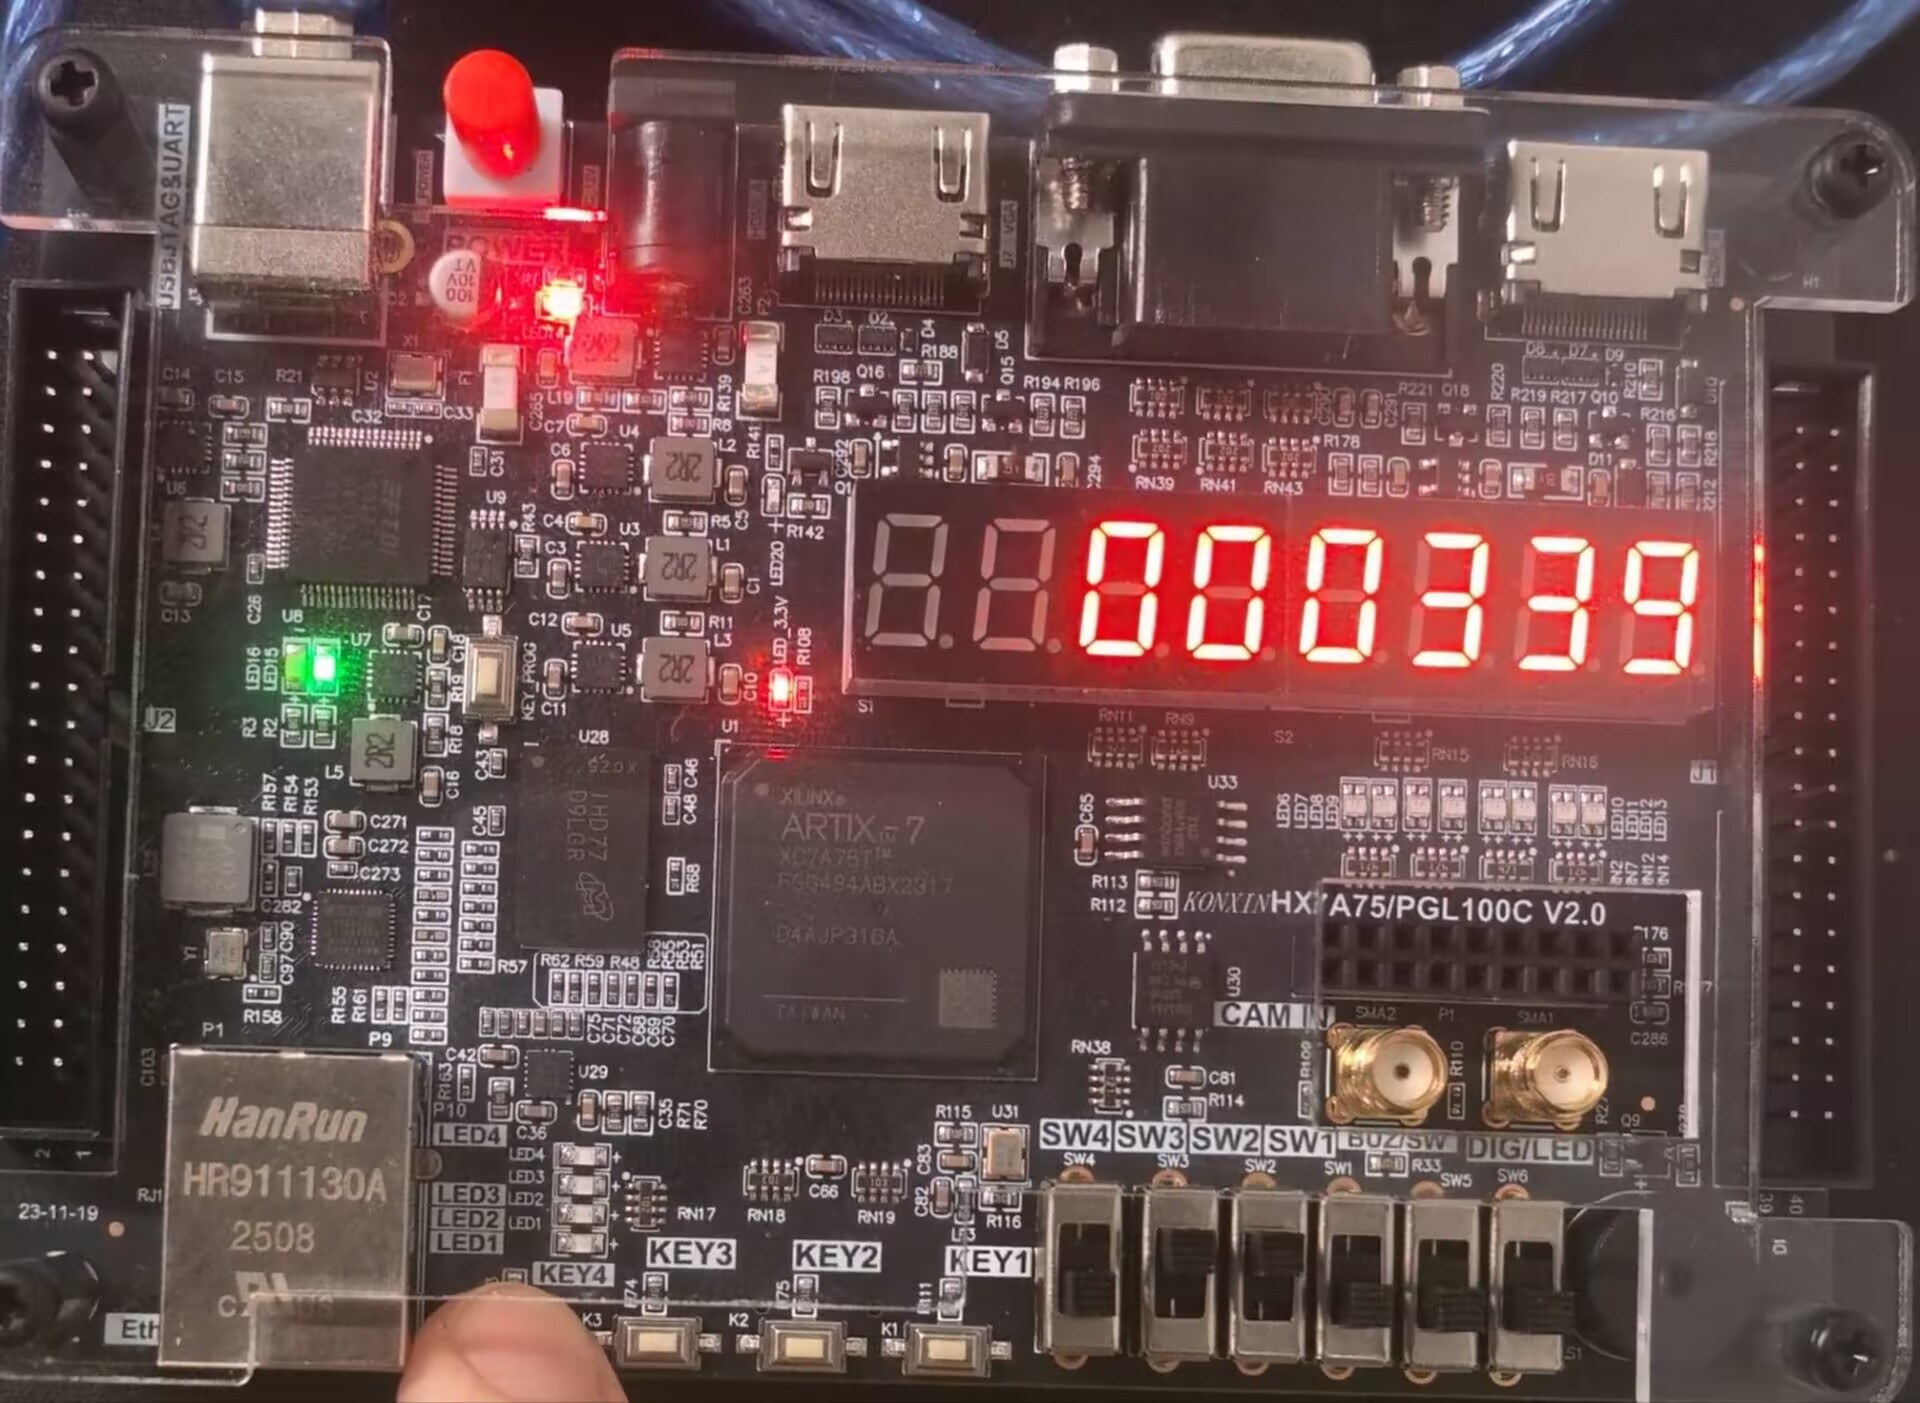
\includegraphics[width=\linewidth]{复位时000339.jpg}\\[-1mm]
        \scriptsize (a) 复位前 \signal{00:03:39}
    \end{minipage}\hfill
    \begin{minipage}[t]{0.23\textwidth}
        \centering
        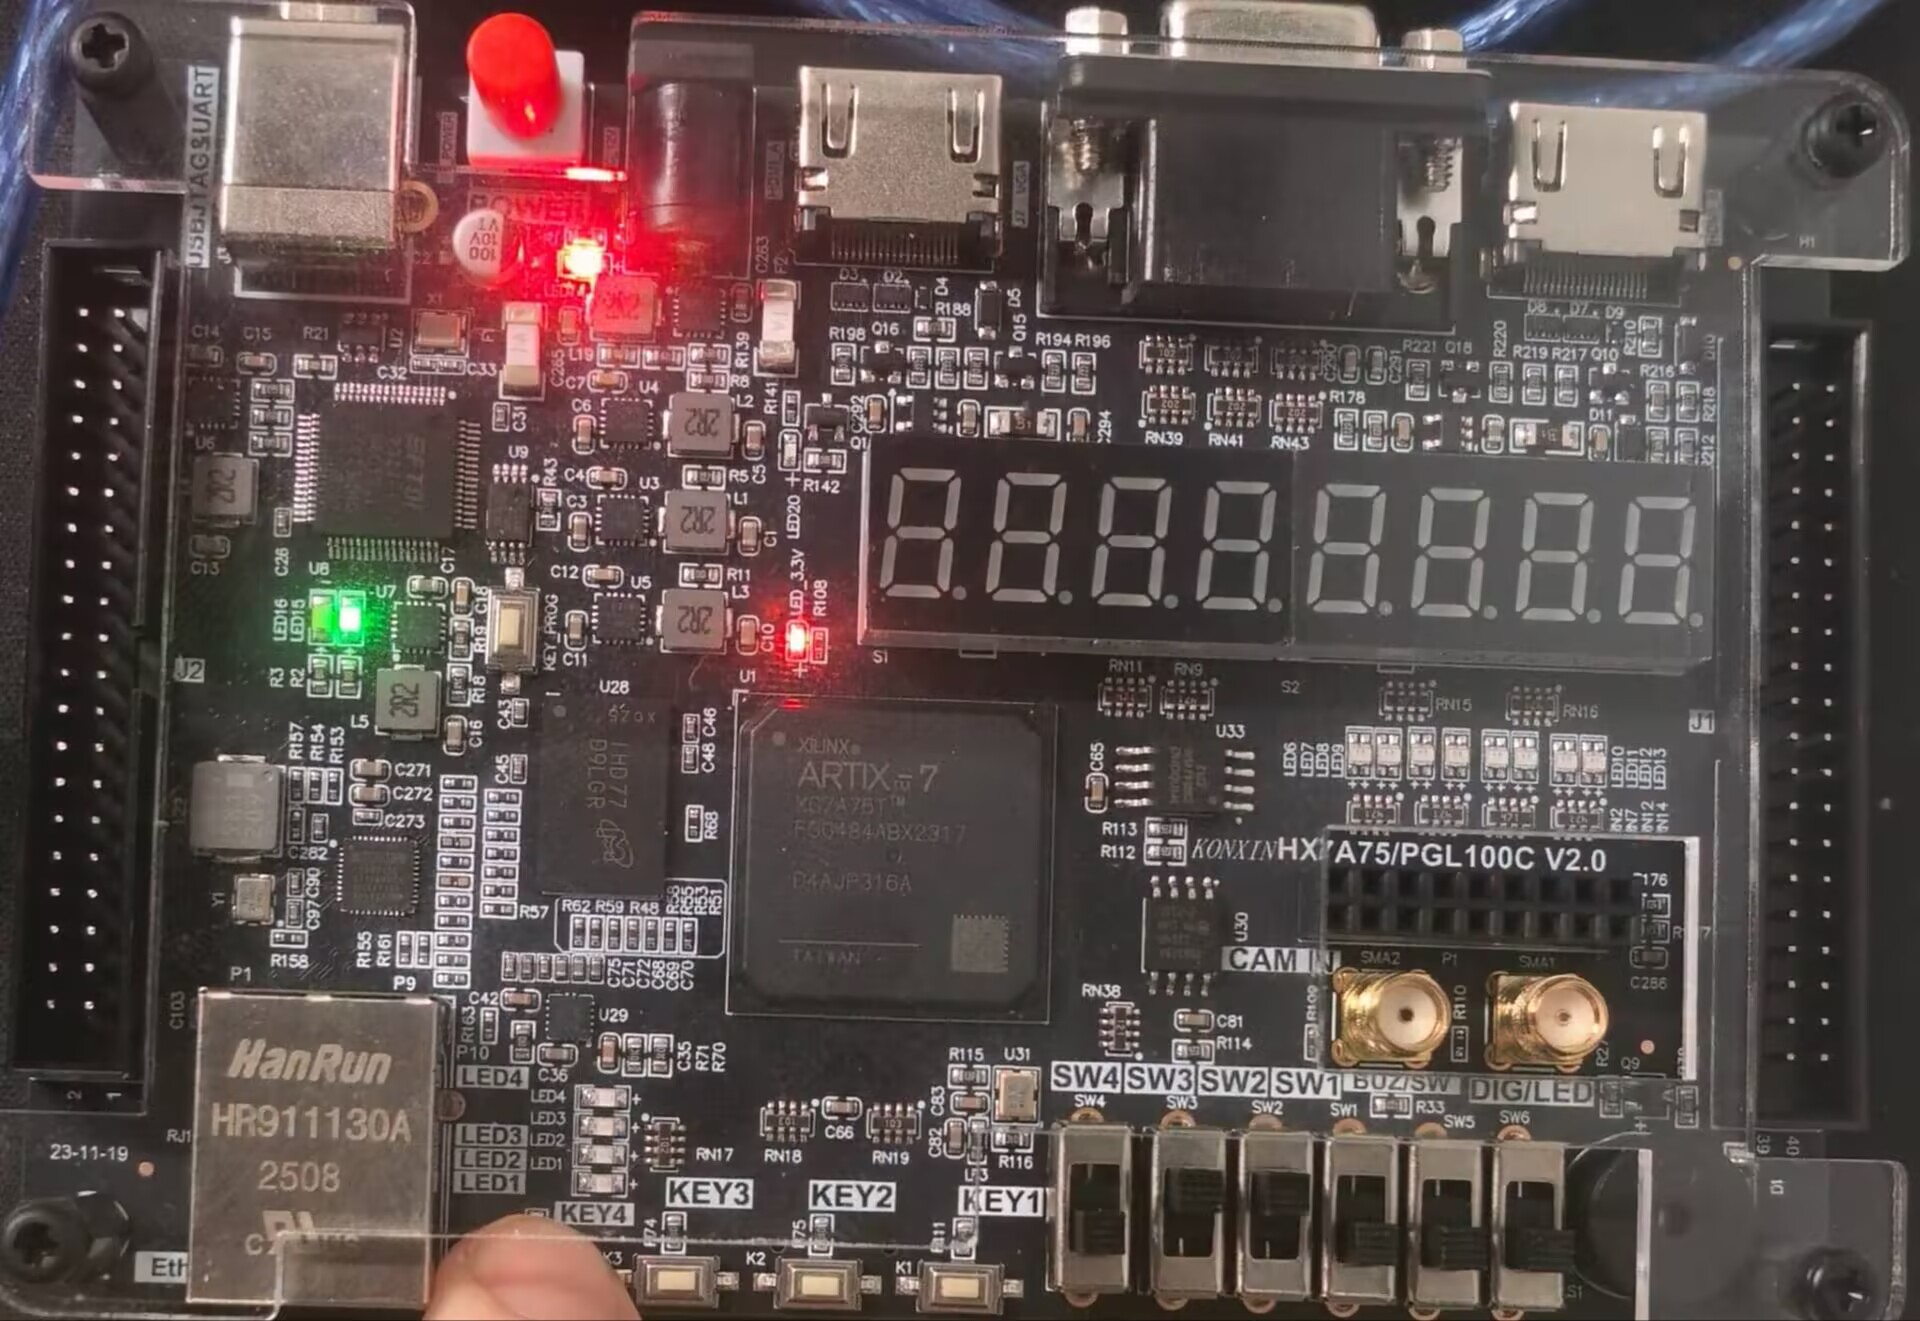
\includegraphics[width=\linewidth]{复位中数码管全灭.jpg}\\[-1mm]
        \scriptsize (b) 数码管全灭
    \end{minipage}\hfill
    \begin{minipage}[t]{0.23\textwidth}
        \centering
        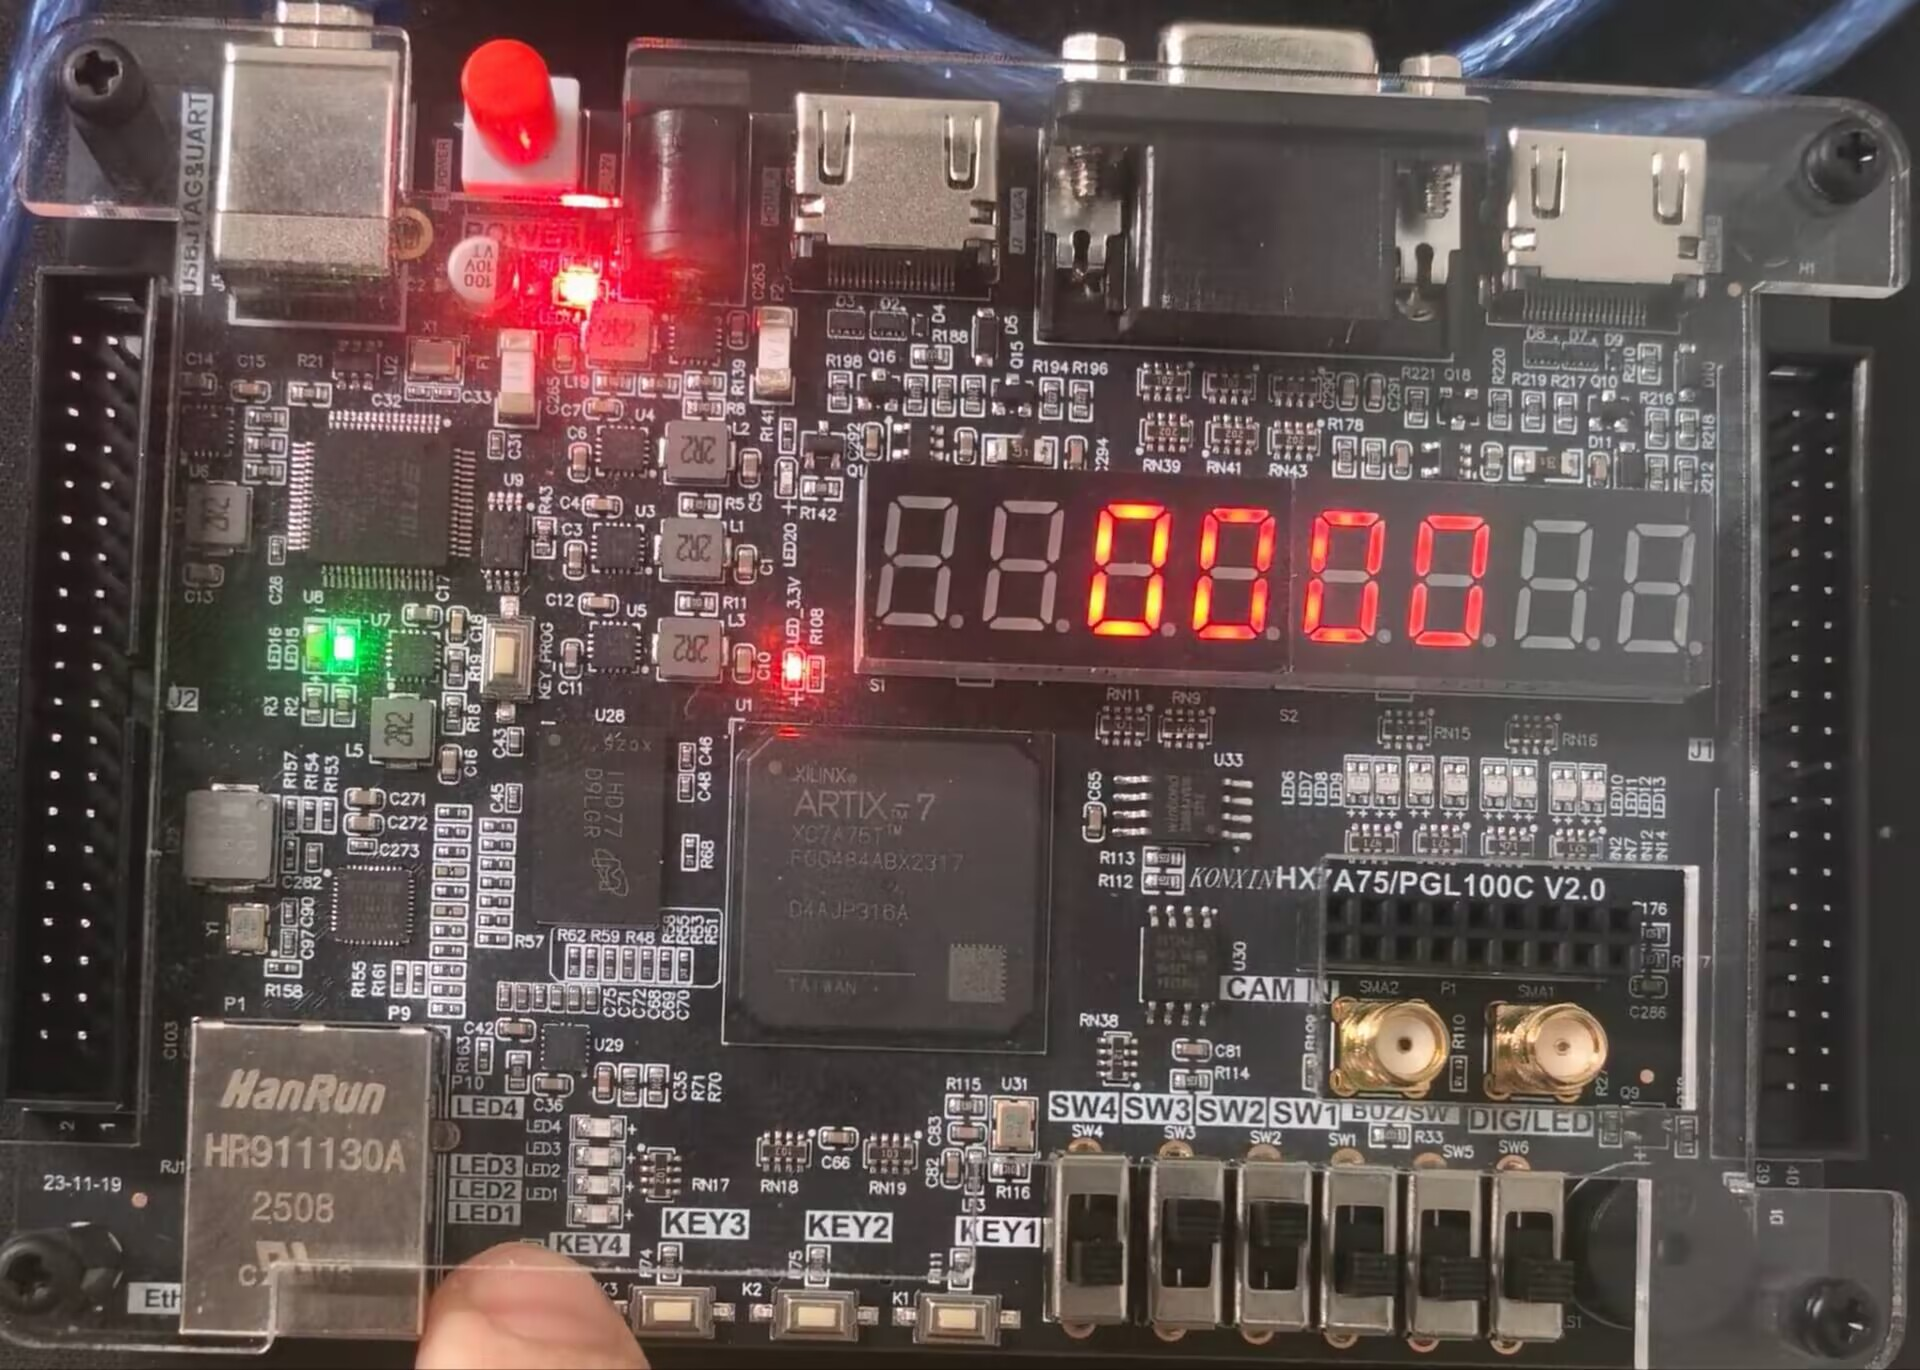
\includegraphics[width=\linewidth]{复位中数码管亮起一半亮起0000__.jpg}\\[-1mm]
        \scriptsize (c) 扫描恢复
    \end{minipage}\hfill
    \begin{minipage}[t]{0.23\textwidth}
        \centering
        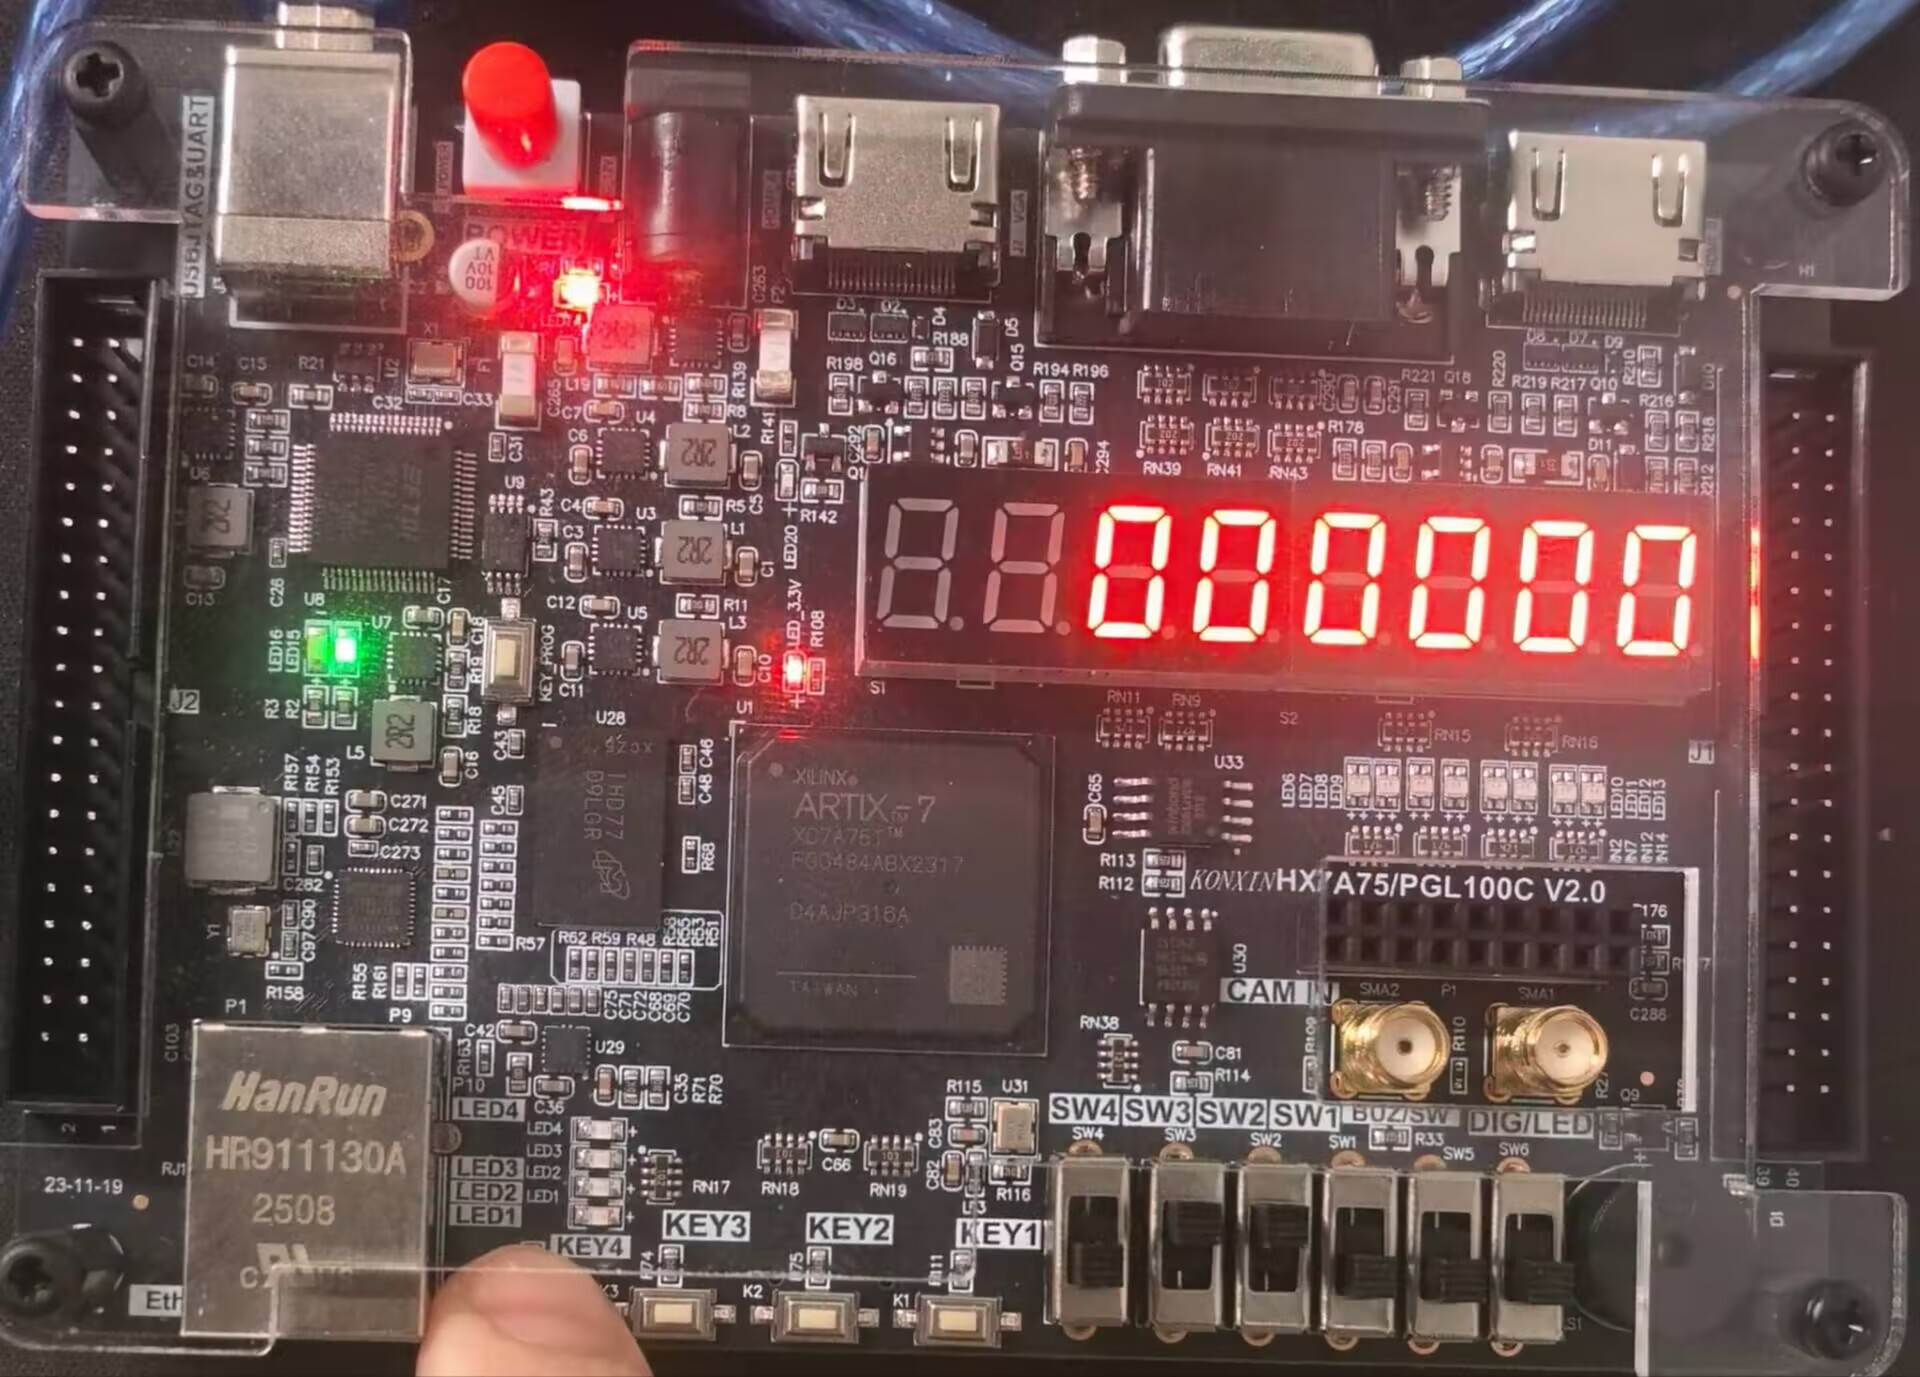
\includegraphics[width=\linewidth]{复位完毕亮起000000.jpg}\\[-1mm]
        \scriptsize (d) 复位完成 \signal{00:00:00}
    \end{minipage}
    \caption{全局复位的板级状态变化过程}
    \label{fig:board-reset}
\end{figure}

\section{分工说明}

\begin{longtable}{@{}clp{12cm}@{}}
    \caption{分工说明}\label{tab:division}\\
    \toprule
    序号 & 组员 & 负责内容 \\
    \midrule
    \endhead
    1 & 杨天宇 & 分频器、按键消抖、时间模块、日期模块、仿真验证 \\
    2 & 杨屹立 & 闹钟模块、倒计时模块、控制模块、数码管模块、LED 模块 \\
    3 & 共同 & 约束文件、板级验证 \\
    \bottomrule
\end{longtable}

\appendix
\section{附件说明}

本报告与源代码一同压缩提交。

\begin{longtable}{@{}L{1.2cm}L{5.0cm}L{8.0cm}@{}}
    \caption{源代码文件表}\label{tab:source-code}\\
    \toprule
    序号 & 文件名称 & 说明 \\
    \midrule
    \endfirsthead
    \toprule
    序号 & 文件名称 & 说明 \\
    \midrule
    \endhead
    1 & \signal{clk_div.v} & Verilog：时钟分频模块 \\
    2 & \signal{key_driver.v} & Verilog：按键消抖模块 \\
    3 & \signal{time.v} & Verilog：时间计数模块 \\
    4 & \signal{date.v} & Verilog：日期计数模块 \\
    5 & \signal{alarm.v} & Verilog：三组闹钟模块 \\
    6 & \signal{countdown.v} & Verilog：倒计时模块 \\
    7 & \signal{control_unit.v} & Verilog：控制模块 \\
    8 & \signal{digital_tube.v} & Verilog：数码管显示模块 \\
    9 & \signal{led.v} & Verilog：LED 提醒模块 \\
    10 & \signal{clock_top.v} & Verilog：顶层模块 \\
    11 & \signal{clock_tb.v} & 仿真：系统测试代码 \\
    12 & \signal{clock.xdc} & 约束：管脚与电平配置 \\
    \bottomrule
\end{longtable}

\end{document}
